\chapter{SFCDecomp: Multicriteria Optimized Tool Path Planning in 3D Printing using Space-Filling Curve Based Domain Decomposition in a Graphical Framework}

\section{Introduction}
  We study {\it dense infill} 3d printing problems, where a given region is completely covered by depositing material with an extruder.
  Design of the tool path, i.e., the sequence in which the extruder moves while depositing material, has crucial implications on print quality as well as mechanical properties of the printed object.
  %\delete{In particular, poor tool paths could contribute to print failures, especially in large scale 3d printing.}
  The extruder can go over non-print or previously printed regions with idle movements.
  Two problems closely related to 3d printing are milling and lawn mowing.
  But in the milling problem, the cutter cannot exit the region (pocket) that it has to cover.  
  The lawn mowing problem is similar to 3d printing problem since the cutter can mow over non grass as well as already mowed regions.
  But one wants to minimize non-print movement in 3d printing in order to improve efficiency.
  
  Various geometric tool path patterns are used such as zigzag, spiral, and contour parallel, but most of them suffer from directional bias.
  For instance, spiral and contour parallel tool paths do not allow cross weaving between adjacent layers.
  More generally, aspects of tool path design across multiple layers and their effects on mechanical properties of the printed objects have not been studied in detail.
  This motivated the development of our framework for optimization based tool path planning, where we can optimize the tool path based on multiple criteria.
  At the same time, we show that the 3d printing tool path optimization problem is NP-hard, and hence large instances become much harder to solve.
  One approach to handle large instances involves decomposition into subdomains, where the subproblems can be solved in parallel and the overall tool path designed by combining solutions for the subdomains.

\subsection{Our Contributions}
  We focus on the minimum turn, minimum edge cost, as well as combinations of these two 3d printing problems.  
  \begin{itemize}
    \item We show that minimum turn cost 3d printing problem is NP-hard, even when the region is a simple polygon.  
    \item We develop \emph{SFCDecomp}, a space filling curve based decomposition framework to solve large instances of 3d printing problems efficiently by solving subproblems from the decomposition independently.
      Our framework builds toolpaths over a total of 799,716 nodes across 169 layers for the Buddha, and over 812,733 nodes across 360 layers for the Bunny.
      See Figures \ref{fig:introimage} and \ref{fig:bunnybuddha} for sample layers and a print.

    \item Building on SFCDecomp, we develop a multicriteria optimization approach for toolpath planning.
      We demonstrate the utility of this approach by maximizing or minimizing tool path edge overlap between adjacent layers, while jointly minimizing turn costs.
    \item We measure the mechanical strength of prints with varying tool path edge overlaps across adjacent layers.
      Strength testing of tensile test specimens printed with tool paths that respectively maximize and minimize adjacent layer edge overlaps reveal significant differences in tensile strength between the two classes of prints.      
  \end{itemize}

\begin{figure}[hbp!] 
  \centering
  %\bigskip
  %\includegraphics[height=2.1in]{BunnyLayer_124.png} %bunnyLayer_124_image_256}
  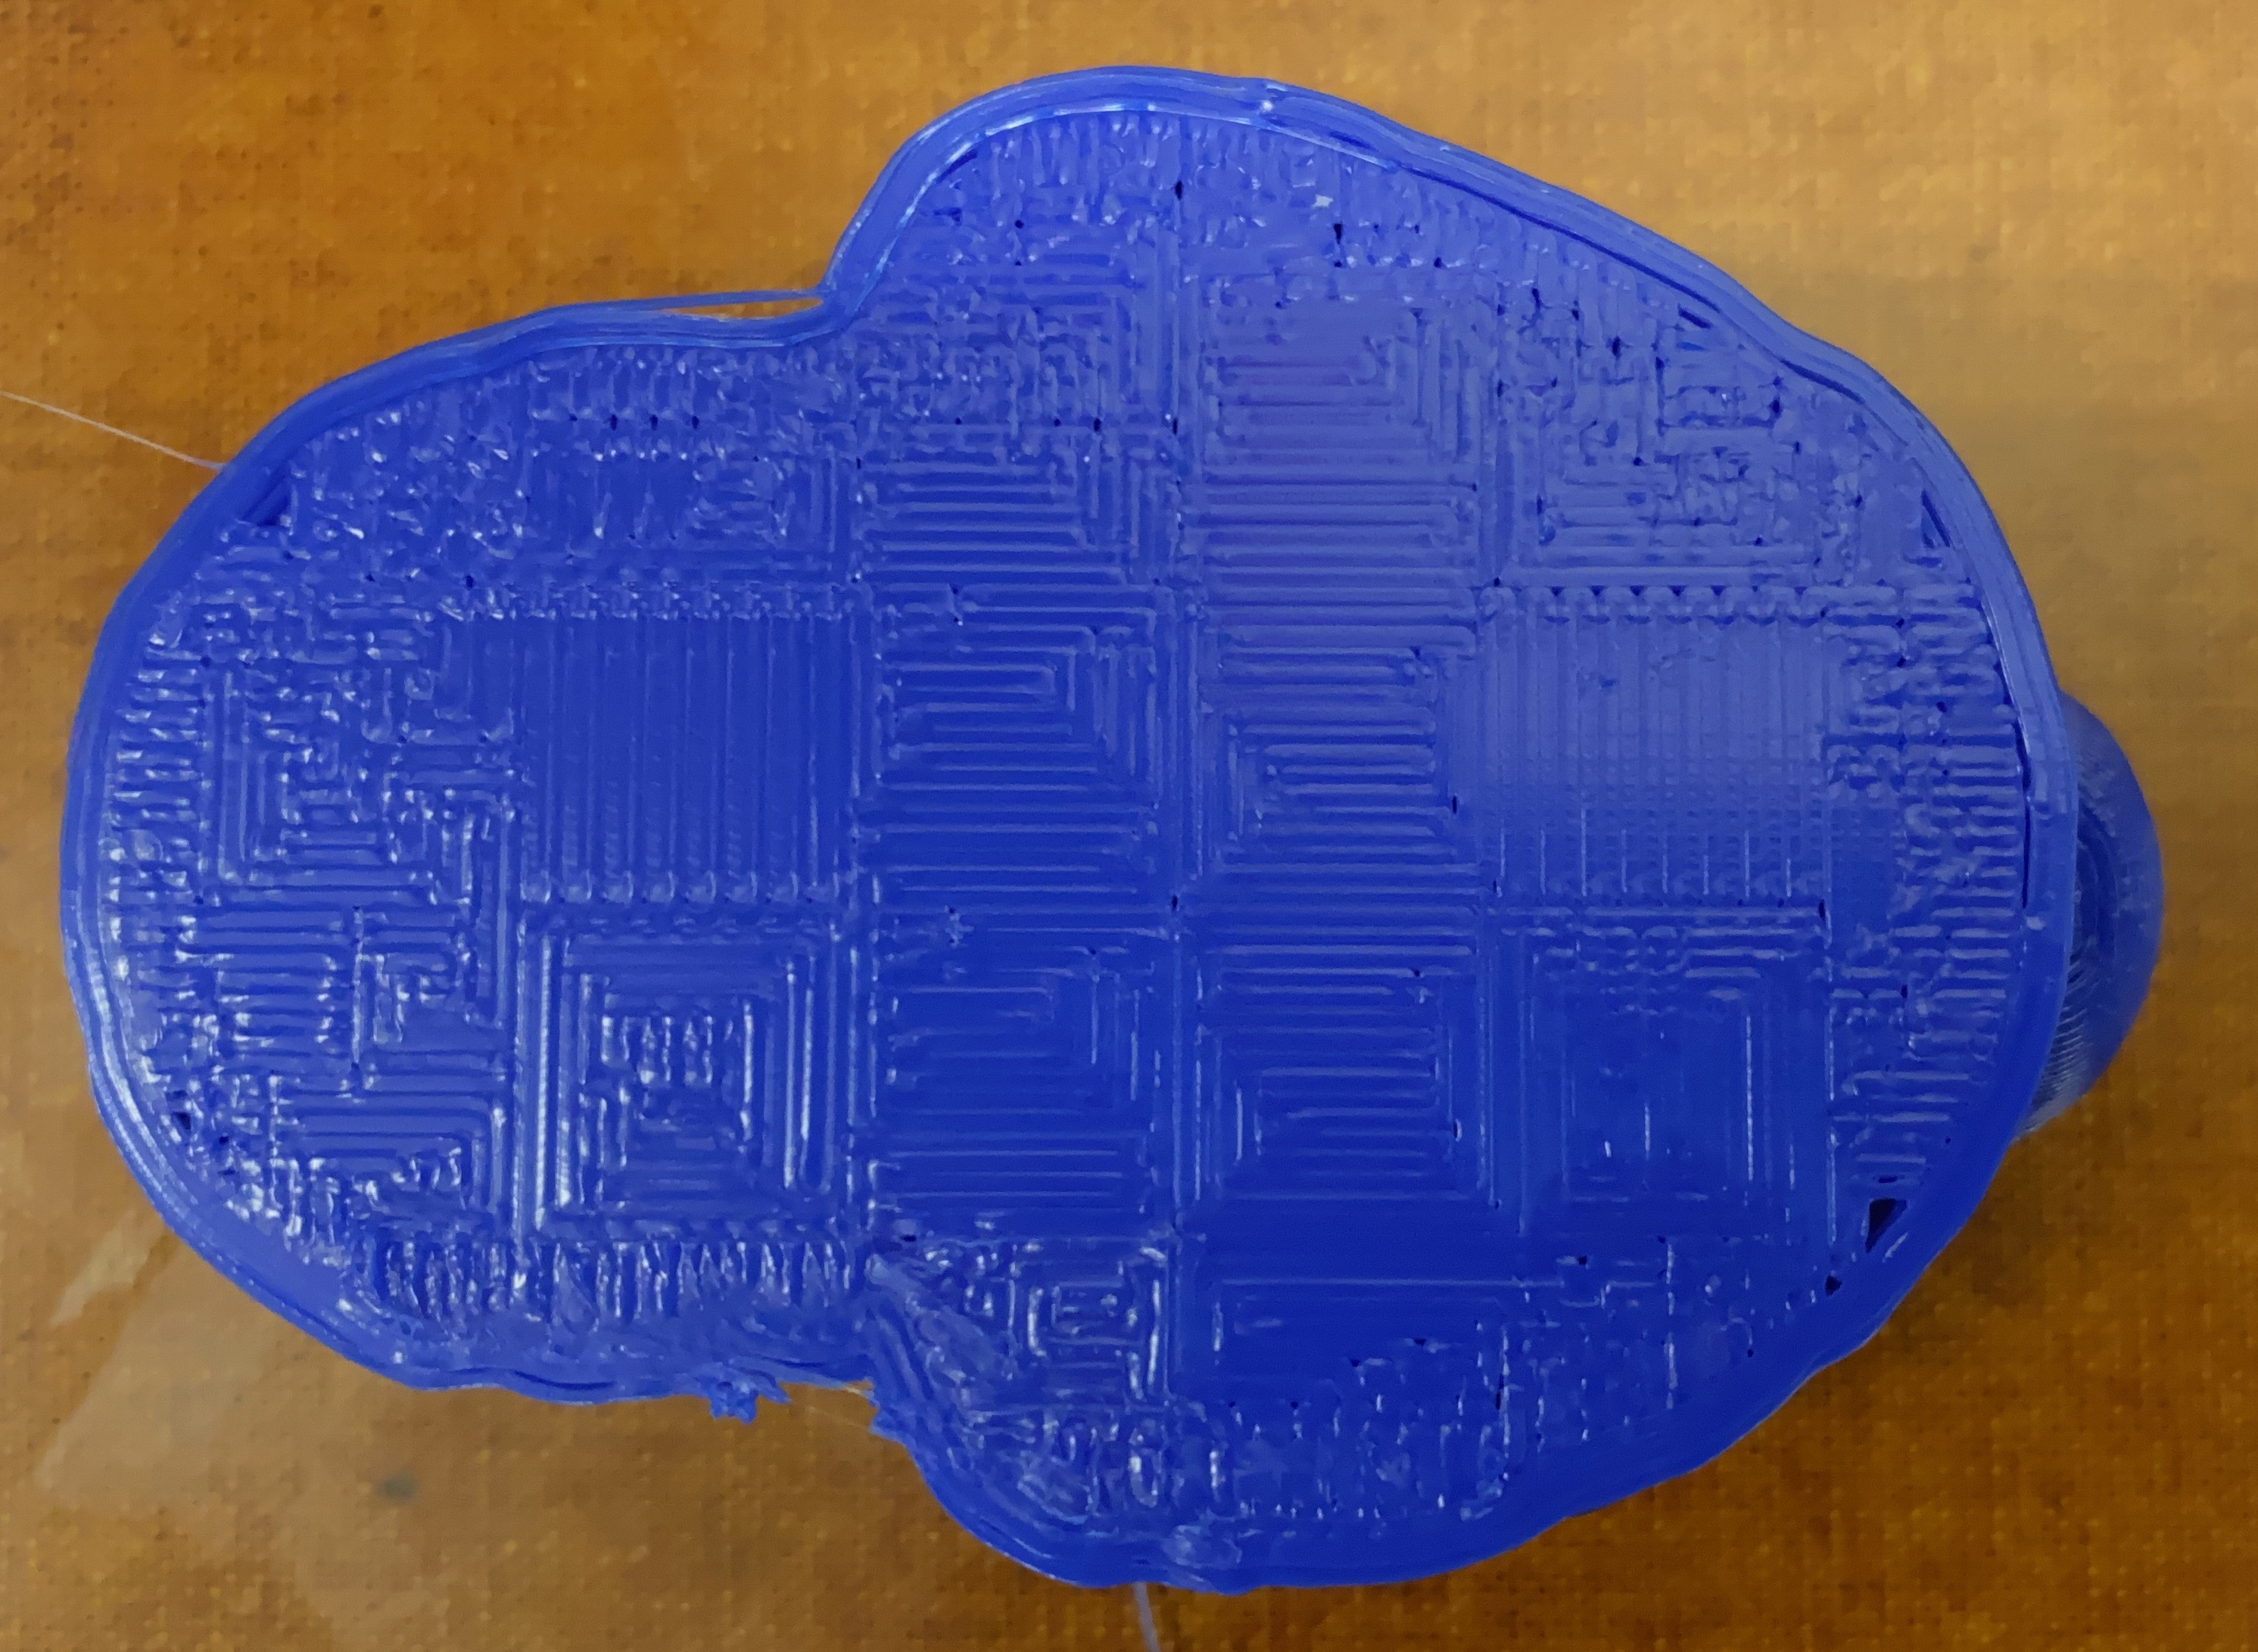
\includegraphics[width=3.2in]{layer124_01.JPG}
  \\
  \bigskip
  %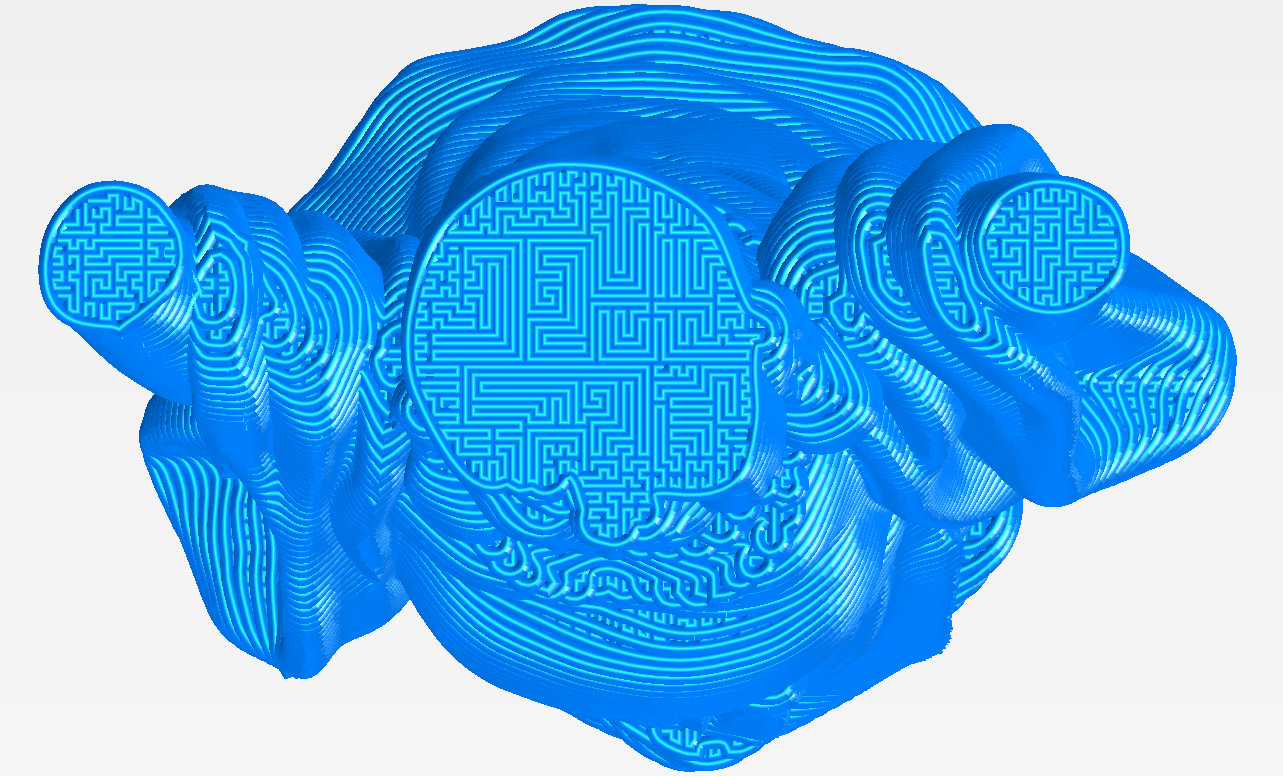
\includegraphics[height=1.86in]{BuddhaTopImageLayer_138_256}
  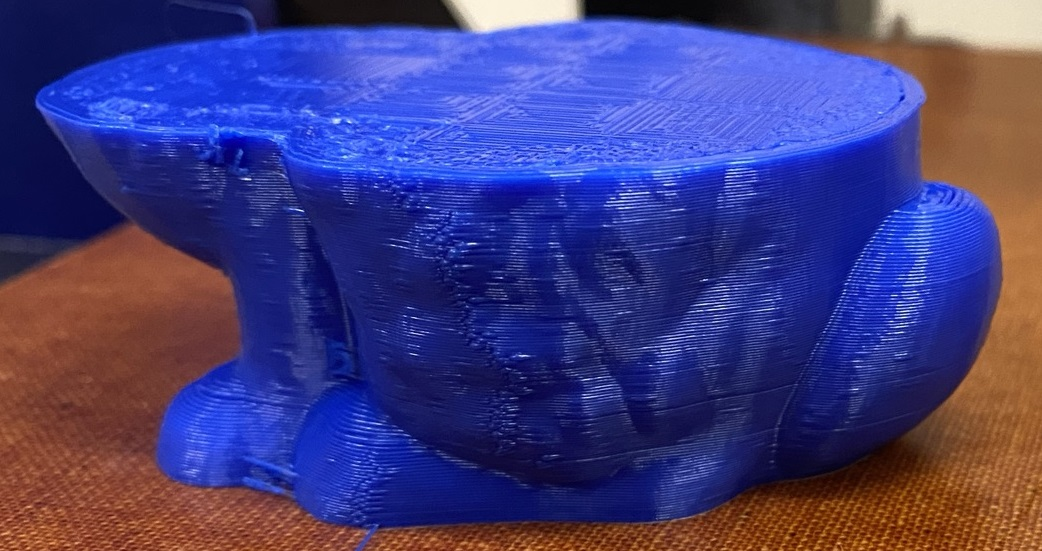
\includegraphics[width=3.2in]{layer124_side.JPEG}
  \caption{\label{fig:introimage} Top and side views of a print of the Bunny at Layer 124.}  	
\end{figure}
  

\subsection{Related Work} \label{sec:previouswork}

The lawn mowing, milling, and 3d printing problems are closely related to the more general geometric traveling salesman problem (TSP).

  \paragraph{Geometric TSP} \label{sec:geometricTSP}
  In the geometric traveling salesman problem (GTSP) with mobile clients, the objective is to find an optimal tour of the salesman to visit a given set of clients, each of whom can travel up to a distance $r$ to meet the salesman.
  Variants of the GTSP include the milling and lawn mowing problems. 
  %3dPP in general is closely related to lawn mowing problem with no re-mowing, where instead of removing we are adding material. 
  %In general lawn mowing problem is NP-hard \cite{Em1993}. 
  Arkin et al.~\cite{ArFeMi2000} showed that the minimum length lawn mowing problem for polygonal regions with or without holes is NP-hard, and the minimum length milling problem for polygon regions with holes is also NP-hard.
  Arkin et al.~\cite{ArBeDeFeMiSe2005} also showed that the minimum turn milling problem is NP-hard.  
  %Minimum length lawn mowing problem for simple polygonal region basically is Hamiltonian circuit problem (HCP) on a solid grid graph(without holes). 
  %It has been shown that HCP for square and triangle solid grid graph can be solved in polynomial time\cite{WiCh1997,EmAnKaHeJoYuVaDaHe2009}.
  
  The TSP with turn costs is known as the \emph{angular metric TSP}.
  Aggarwal et al.~\cite{AgCoKhMoSc2000} proved it is NP-hard. 
  %and gave $O(log(n))$ approximation algorithm. 
  Integer programming formulations of this problem are hard to solve to optimality \cite{AiAnFrJUlAl2017}. 
  Finding a tour connecting a given set of points such that angles between two adjacent edges of the tour is constrained was studied by Fekete and Woeginger \cite{FeWo1997}. 
  Reif and Wang \cite{ReWa1998} showed that the angle restricted shortest path problem with obstacles is NP-hard.
  In 3d printing, apart from computational challenges (NP-hardness), the optimal print direction can change based on mechanical factors such as temperature gradient to minimize thermal residual stress and strain.
  This aspect is a direct motivation for developing our framework.
  %Milling problem with Turn cost is NP-complete even for rectilinear pockets and cutter moves axis parallel \cite{ArBeDeFeMiSe2005}.
  %Polynomial time algorithm for minimum turn milling for simple orthogonal polygon is still an open problem \cite{ArBeDeFeMiSe2005}.
  %In Arc routing problem(ARP) aim is to find least-cost traversal of a specified subset of arcs in a graph may have some constrains. 
  %Chinese postman problem (CPP) and windy postman problem (WPP) are some of the arc routing problems.  
  %Most important property for a graph $G$ for CPP and WPP is \textit{eulerian}.A undirected graph $G$ is Eulerian, if each vertex in $G$ is connected to even number of edges. 
  %CPP(minimum length) algorithms are basically divided into two parts. 
  %First, to find \textit{minimum cost augmentation} that is least cost set of arcs that makes the graph Eulerian.
  %Second, traverse edges of augmented graph, that can be determined in polynomial time. 
  %Since G is an undirected graph is easily solvable. 
  %Augmented  graph can be obtained by solving matching problem \cite{Ja1973} in polynomial time. 
  %CPP(minimum length) can be solved in polynomial time. 
  %To determine least cost traversal of arcs for WPP(minimum length) is NP-hard as shown in \cite{Gu1984, Pe1981} but if $G$ is Eulerian then this problem can be solved in polynomial time \cite{Za1989}.
  %Turn-weighted CPP is NP-complete, since it is basically a TSP on a line Graph $L(G)$ with turn cost at any vertex in $G$, which is equivalent to finding a hamiltonian cycle in a line graph $L(G)$ is NP-complete \cite{ArBeDeFeMiSe2005}.
  %A special case of 3dPP is related to Chinese postman problem (CPP) and windy postman problem(WPP) are arc routing problems related to our work.
  %Prashant et al.~. \cite{} has developed an approach to transform any planar graph satisfying certain conditions into a eulerian planar graph in polynomial time, if graph modification is allowed.
  
  \paragraph{Tool Path Geometry}\label{sec:extruderpath}
  A popular tool path generation method uses zigzag patterns. 
  Space filling curves (SFCs) are also used in generating infill.
  An SFC in 2D is a continuous curve with positive Jordan content (i.e., area $>0$). 
  In 3d printing, the extruded bead has finite thickness and hence length of the SFC is finite. 
  Zhao et al.~\cite{ZhGuHuGaYoChBeZhCoDaBa2016} developed a Fermat Spiral infill (SFC) based smooth tool path optimized for continuity. 
  Contour parallel tool paths follow the boundary of the polygon \cite{YaLoFuWa2002}.
  Although both these methods give curved tool paths, the Fermat Spiral infill \cite{ZhGuHuGaYoChBeZhCoDaBa2016} is smoother.
  Curved tool paths in FDM are usually approximated by piecewise linear line segments.
  Hence highly curved tool paths require increasingly short line segments in the linear approximation.
  %Further, linear approximation of curved tool paths leads to speed and acceleration discontinuities.
  %These discontinuities result in dimensional inaccuracies, seemingly due to lack of synchronization between speed and acceleration \cite{ErYuAl2018}.
  Zhao et al.~\cite{ZhGuHuGaYoChBeZhCoDaBa2016} discussed this limitation of their method for lower end 3d printers.
  They also pointed out that both spiral and contour parallel infills suffer from directional bias due to which adjacent layers cannot cross-weave at an angle.
  This gives zigzag tool paths some advantages over spirals and contour parallel tool paths since zigzag consists of linear segments and allows cross weaving between adjacent layers.

  Kuipers et al.~\cite{KuWuWa2019} developed \emph{CrossFill}, an approach based on SFCs to generate continuous paths for \emph{sparse} infill 3d printing.  
  %\delete{We can observe all of these geometric infill pattern impose restrictions on the tool path.}
  Wasser et al.~\cite{WaJaPi1999} suggested fractal-like SFC for infill based on a TSP heuristic, but their method cannot handle turn costs and have ambiguity on the input graph for general polygons.
  Bertoldi et al.~\cite{BeYaPiGu1998} proposed a method that uses domain decomposition with a classical SFC (Hilbert curve) to find the tool path.
  %\delete{The main advantage of this method is assigning the contour independently in each decomposed domain, which allows more control on the internal microstructure and thermal management to maximize strength.}
  But the Hilbert curve imposes restrictions on print directions.
  In our framework, we use a quadtree for domain decomposition and classical SFC (Hilbert curve) to create sequences of these domains.
  We then employ optimization that could be based on multiple criteria to find the tool path in each decomposed subdomain. 

  \paragraph{Tool Path Optimization}\label{sec:optimization}
  The tool path in each layer can go straight or take turns (within the plane) to fill the layer, and its overall shape affects various quality factors.
  One often tries to optimize the tool path in each layer for its continuity, smoothness, or both.
  But optimizing for multiple quality factors at one time could be highly inefficient.
  For instance, spiral and contour parallel infills try to optimize smoothness and continuity of the tool path, but cannot consider cross weaving between layers due to directional bias \cite{GiRoSt2015}.
  Lensgraf, Mettu, and coauthors \cite{LeMe2016,LeMe2017,LeMe2018,YoLeFiClMe2020} have used graphical frameworks based on search algorithms, but do not include costs for change in direction.
  In contrast, our graphical cost-based optimization framework for complete infill problems can model new quality factors by varying the edge costs, and also models turn costs.
  In fact, our graphical optimization framework can employ user-defined costs that capture any quality factor.
  %Note: Continuity of tool path is  considered locally governed by space filling curves not by optimization
  
  \paragraph{Domain Decomposition}\label{sec:domaindecomposition}
  The geometric TSP is NP-hard \cite{Pa1977}.
  An alternative approach is to use domain decomposition, solve a TSP for the infill in each subdomain, and then connect the individual subdomain paths. 
  Chazelle and Palios \cite{ChPa1994} presented a review of some decomposition strategies.
  Convex decomposition of polygons is a well studied problem, e.g., see the book by Keil \cite{Ke2000}. 
  Exact convex decomposition for simple polygons without holes can be computed efficiently \cite{ChDo1979,ChDo1985}, but is NP-hard for polygonal regions with holes \cite{AnMoEr1982}. 
  An alternative can be to do approximate convex decomposition \cite{LiAm2006}.
  
  Domain decomposition has been used in 3d printing applications \cite{DwKo2004,DiPaCuLi2014,JiHeFuZhDu2017} to subdivide the polygon into sub-polygonal regions and find a cycle for each sub-polygon using closed zigzag curves to cover most of the vertices in them, and then join these cycles to find a complete tour.
  But their geometric decomposition does not guarantee existence of feasible dual graph of each sub-polygon, whereas our decomposition approach guarantees existence of dual pixel graph of each sub-polygon.
  %\delete{However each cycle is a strictly closed zig-zag curve, and the existence of a cycle that covers the sub-polygon for a given size of extruder is not guaranteed.}
  %\delete{Further both methods do not work properly with smooth concave boundaries.}
  %\delete{Also, joining more than two cycles to get a complete tour changes neighborhoods of vertices visited in a sequence.}
  %\textcolor{blue}{Further, joining more than two cycles to get a complete tour changes neighborhoods of vertices visited in a complete tour as shown in Figure \ref{}. Hence we will primarily focus on finding paths and connecting them to get a complete path.}
  We will primarily focus on finding paths and connecting them to get a complete path, but our work can be extended to finding complete tour by joining cycles.
  We also guarantee the existence of an optimal connected path in each sub-polygon.
  We can vary the decomposition between alternate layers.
  The complete path generated by our method can have discontinuities \emph{only} at the boundaries of the polygon.
  
  To summarize, in the paragraph on \emph{Tool Path Geometry} we motivated the use of rectilinear tool paths, and that on \emph{Tool Path Optimization} we motivated the use of optimization tools.
  But TSP and variants are NP-hard in general, and that motivated our use of \emph{Domain Decomposition}.
  
  \section{Preliminaries}
Let the extruder $\xi$ be the axis aligned unit square.
$\xi(p)$ denotes the placement of $\xi$ at point $p \in \R^2$ as its center.
The \textit{ {\bfseries Geometric 3d printing problem} (3dPP) on a polygon $R$ is to find a path/tour $\pi$ such that every point in $R$ is covered by the placement of $\xi(p)$ on $\pi$ subject to total idle movement less than or equal to $\epsilon$, where $R \subseteq \cup_{p \in \pi} \xi(p)$ and $\epsilon > 0$, a constant.}
Note that some placement of $\xi(p)$ can hit outside the region $R$.
We consider minimizing total length (sum of edge weights, more generally) or total turn cost, or a combination of both. 
We restrict our attention to integral orthogonal polygonal regions with or without holes, and extruder is a unit square restricted to axis parallel motion.
In a integral orthogonal region all boundary turns are $90^{\circ}$, and boundary vertices have integer coordinates.
It can be considered a union of pixels, i.e., unit squares with axis-parallel edges and integer vertices (see Figure \ref{fig:inteortho3dprintprob}).
Hence we name it the \emph{integral orthogonal $3d$-printing problem} (IO3dPP), and will also refer to it in short as 3dPP.
%There is a special case of IO3dPP problem, where polygonal region do not have a 2x2 square of pixels called thin integral orthogonal 3d printing problem (TIO3dPP) which is quite similar to chinese postman problem(CPP).
We prove that 3dPP is NP-hard. % of  without thin regions
%(i.e., not having any $2 \times 2$ square of boundary pixels).
%for the special case with $\epsilon \leq 1$.  

\begin{figure}[htp!] 
  \centering
  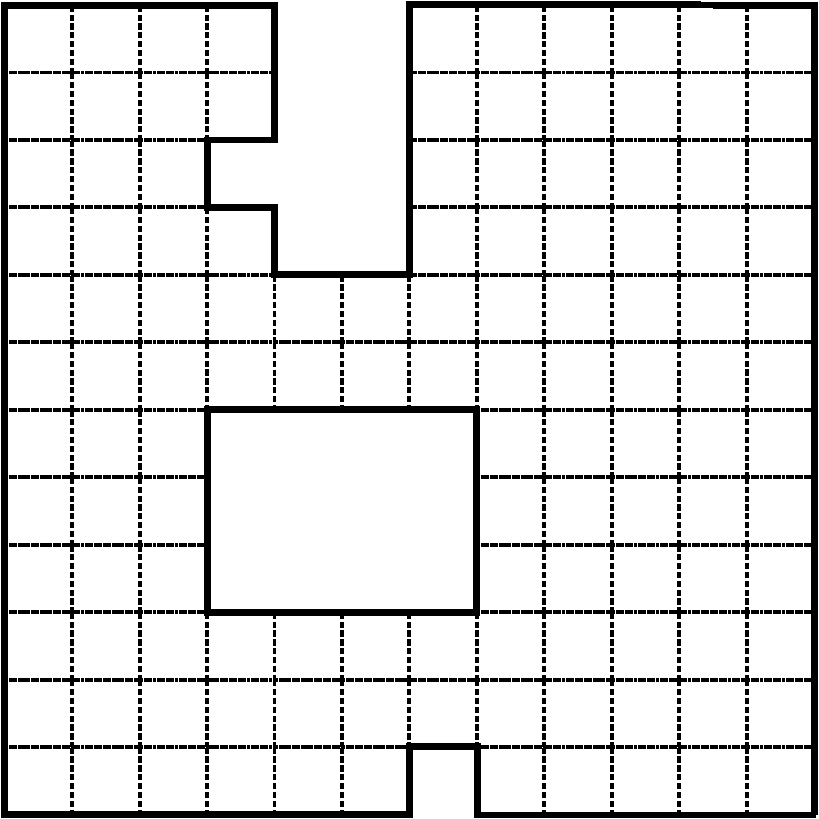
\includegraphics[scale=0.40]{integral_orthogonal_3d_printing_problem_Fig_1_crop}
  \hspace*{0.03in}
  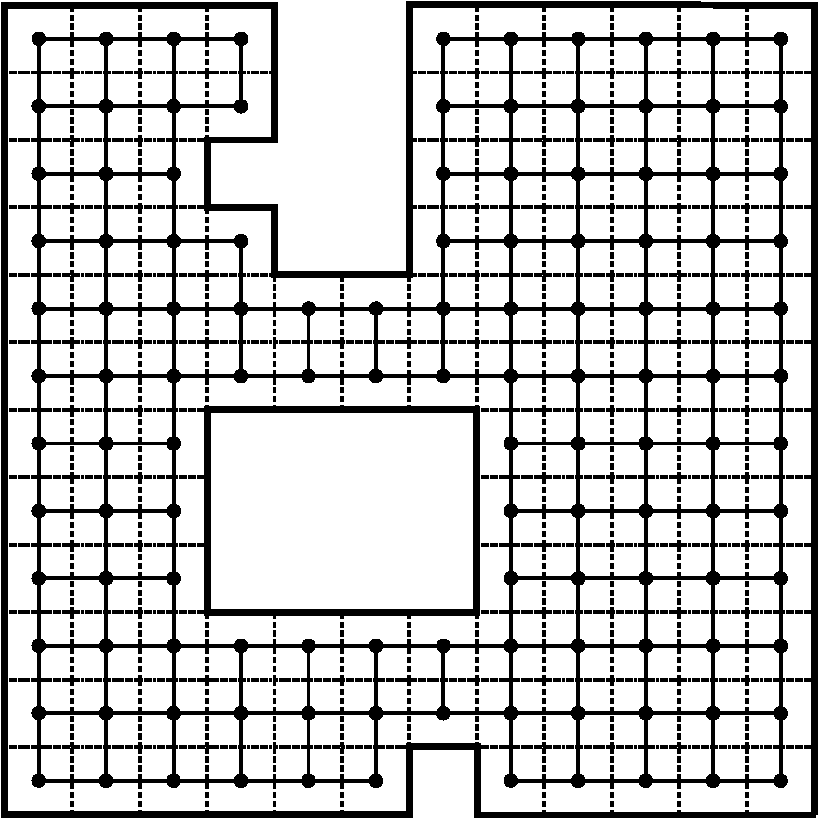
\includegraphics[scale=0.40]{integral_orthogonal_3d_printing_problem_Fig_2_crop}
  \caption{\label{fig:inteortho3dprintprob}
    An integral orthogonal region with a hole (left) and dual graph (right).
  }
\end{figure}


We consider a connected, undirected, planar graph $G=(V,E)$ with $V= \{v_1, \dots, v_n\}$ and $E= \{(v_i, v_j): v_i, v_j \in V \text{ and } i \neq j\}$.
For each edge $(v_i, v_j) \in E$ there is a cost (or weight) $c_{ij}$ that depends on the Euclidean distance between vertices (if $(v_i, v_j) \not\in E$ then $c_{ij} = M$, some large positive value).
We take the \textit{turn cost} at vertex $v_i$ as $c_i = 0$ if the toolpath goes straight through $i$, and $c_i = 1$ if the path makes a turn ($90^{\circ}$). 
%In case of minimum length problem cost($c_{ij}$) is associated with edge length where as in minimum turn problem cost($c_i$) is associated with turn angle.   
For the default Euclidean minimum length problem, $c_{ij}$'s form a metric.
But $c_i$'s for the minimum turn problem do not form a metric \cite{ArBeDeFeMiSe2005}.

\section{NP-hardness proofs}

\subsection{Minimum Length 3dPP}
Itai et al.~\cite{ItPaSz1982} showed that the Hamiltonian circuit problem for grid graphs is NP-complete.
Arkin et al.~\cite{ArFeMi2000} showed that minimum length lawn moving problem for simple polygon or polygon with holes is NP-hard based on reduction from Hamiltonian circuit in planar bipartite graph with maximum degree 3 to Hamiltonian circuit in grid graphs.

\begin{thm} 
  Minimum length 3dPP is NP-hard for any connected polygon $R$ (with or without holes) and axis-aligned unit square extruder. 	
\end{thm}
\begin{proof}
  Proof of Arkin et al.~\cite{ArFeMi2000} for lawn moving problem can be directly adapted to that for 3dPP where there is no idle movement for connected polygon $R$ with or without holes.
  We note that no point in $R$ is mowed more than once in their proof, and for a simple polygon the total idle movement is at most $\epsilon=1$.    
\end{proof}

 
\subsection{Minimum Turn Cost 3dPP}

We use a reduction similar to one introduced by Arkin et al.~\cite{ArBeDeFeMiSe2005}.
First we show Hamiltonicity of unit segment perpendicular end point intersection graph (HUSPEPIG) of axis aligned unit segment is reducible to Hamiltonicity of square grid graph problem.
Unit segment perpendicular end point intersection graphs consist of unit horizontal or vertical segments that intersect only at end points (see Figure \ref{fig:USPIGNC_graph}).

\begin{figure}[ht!]
  \centering
  \begin{subfigure}[t]{2in}
    \centering
    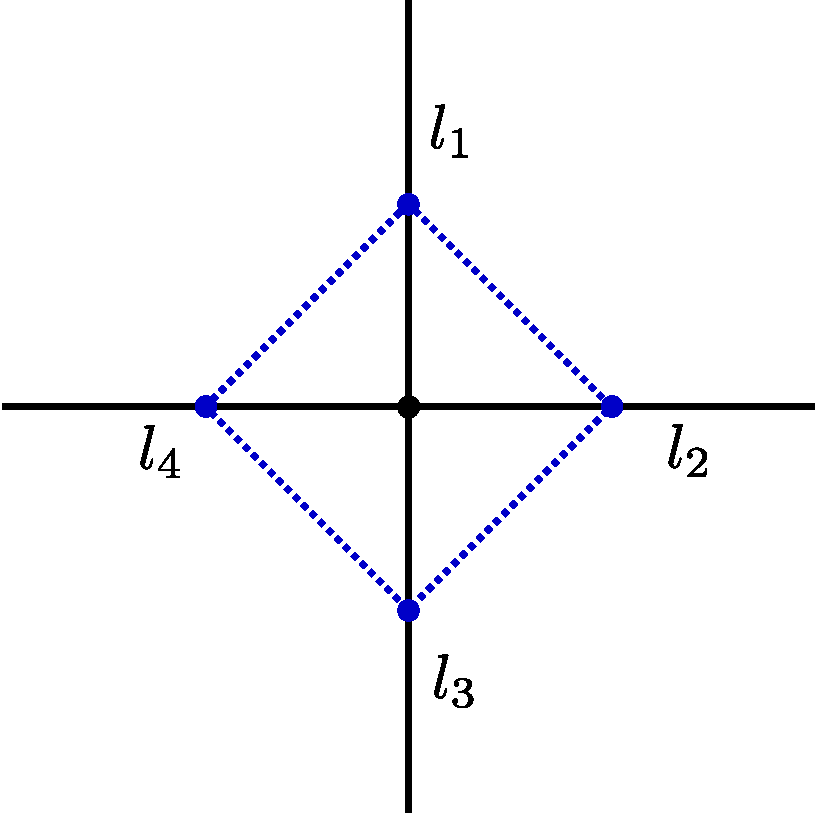
\includegraphics[scale=0.40]{USPIGNC_Fig_1_crop}
    \caption{\label{fig:USPIGNC_grapha}}
  \end{subfigure}
  \quad\quad
  \begin{subfigure}[t]{2in}
    \centering
    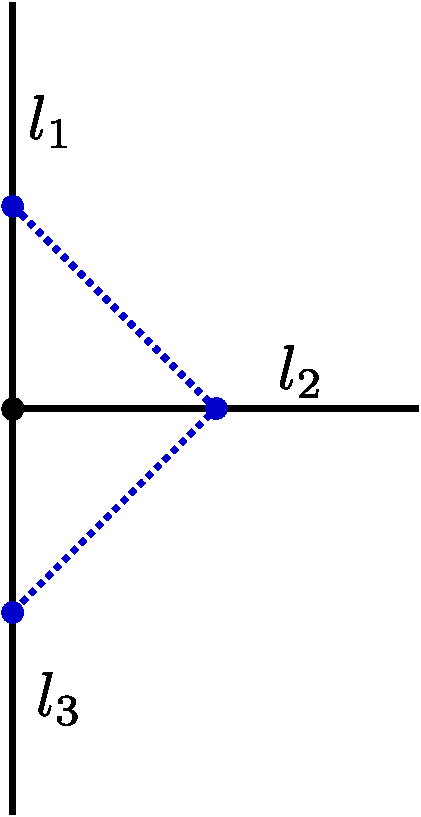
\includegraphics[scale=0.40]{USPIGNC_Fig_2_crop}
    \caption{\label{fig:USPIGNC_graphb}}
  \end{subfigure}	
  \begin{subfigure}[t]{2in}
    \centering
    \vspace*{-1.4in}
    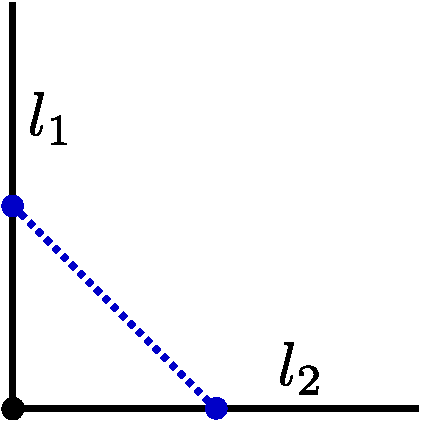
\includegraphics[scale=0.40]{USPIGNC_Fig_3_crop}
    \vspace*{0.4in}
    \caption{\label{fig:USPIGNC_graphc}}
  \end{subfigure}
  \begin{subfigure}[t]{2in}
    \centering
    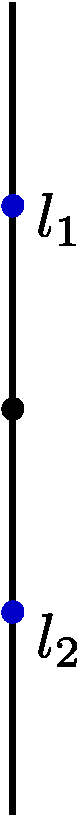
\includegraphics[scale=0.40]{USPIGNC_Fig_4_crop}
    \caption{\label{fig:USPIGNC_graphd}}
  \end{subfigure}
  \caption{\label{fig:USPIGNC_graph} $l_1, l_2, l_3, l_4$ (black) are unit line segments.
    Figures (a), (b), (c), (d) show all possible intersections at the end points.
    Intersection graph (dotted blue lines) of corresponding  intersection of line segments are shown in Figures (a), (b), and (c).
    In Figure (d), unit segments intersect at an end point but are not perpendicular, so no edge is shown in the intersection graph.}
%  \vspace*{-0.4in}
\end{figure}


\begin{lem} 
  Hamiltonicity of square grid graph is reducible to HUSPEPIG.	
\end{lem}

\begin{proof}
  Consider a bipartite grid graph $G$ with vertices having integer coordinates.
  Then $G$ can be represented as $2$-color graph.
  Rotate $G$ by $45^{\circ}$ and scale down edges in $G$ by $\sqrt{2}$.
  The length of each edge in this arrangement is $1/2$, the coordinates of each vertex are integer multiple of $1/2$, and smallest distance between vertices of same color is $1$.
  Assign each white vertex a horizontal unit line segment and each black vertex a vertical unit line segment centered at the vertex to obtain the instance of HUSPEPIG (see Figure \ref{fig:Grid_to_USPIGNC}).
  %Hence HAMILTONICITY of square grid graph is reducible to HUSPEPIG.
\end{proof}

\begin{figure}[ht!]
  %\vspace*{-0.55in}
  \centering
  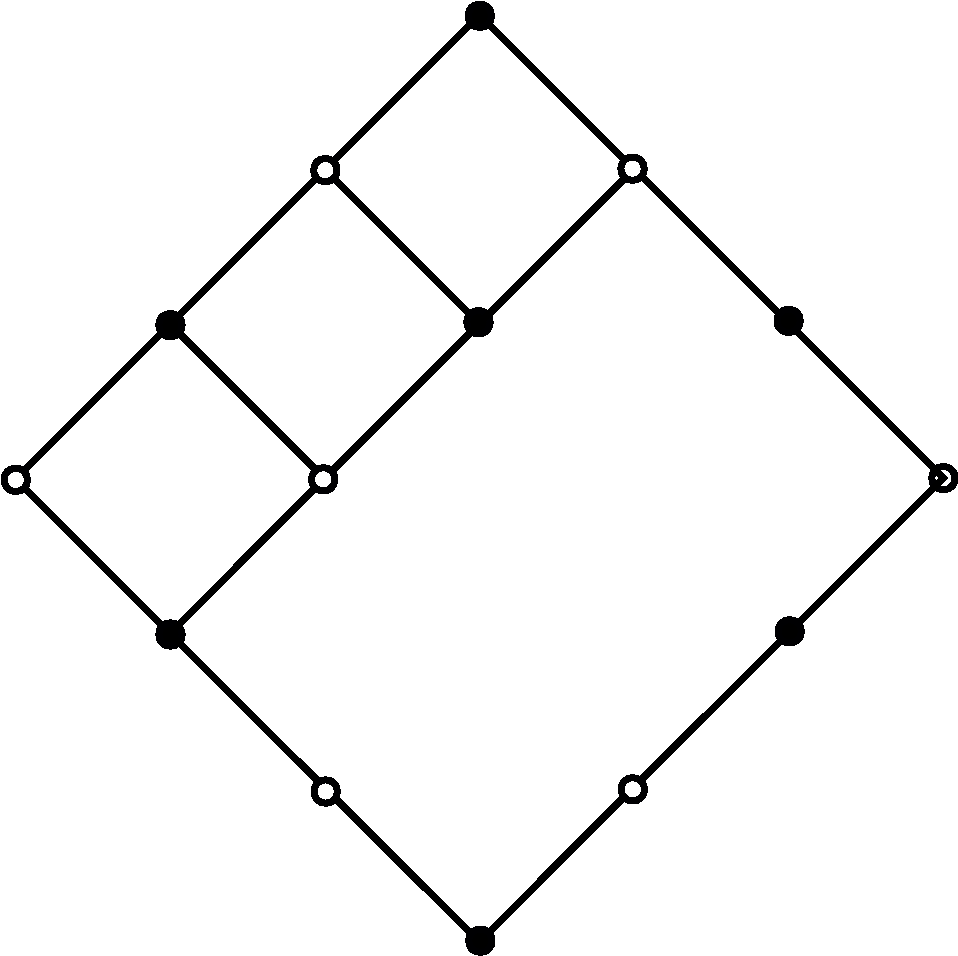
\includegraphics[scale=0.40]{Grid_to_USPIGNC_Fig_1_crop}
  \hfill
  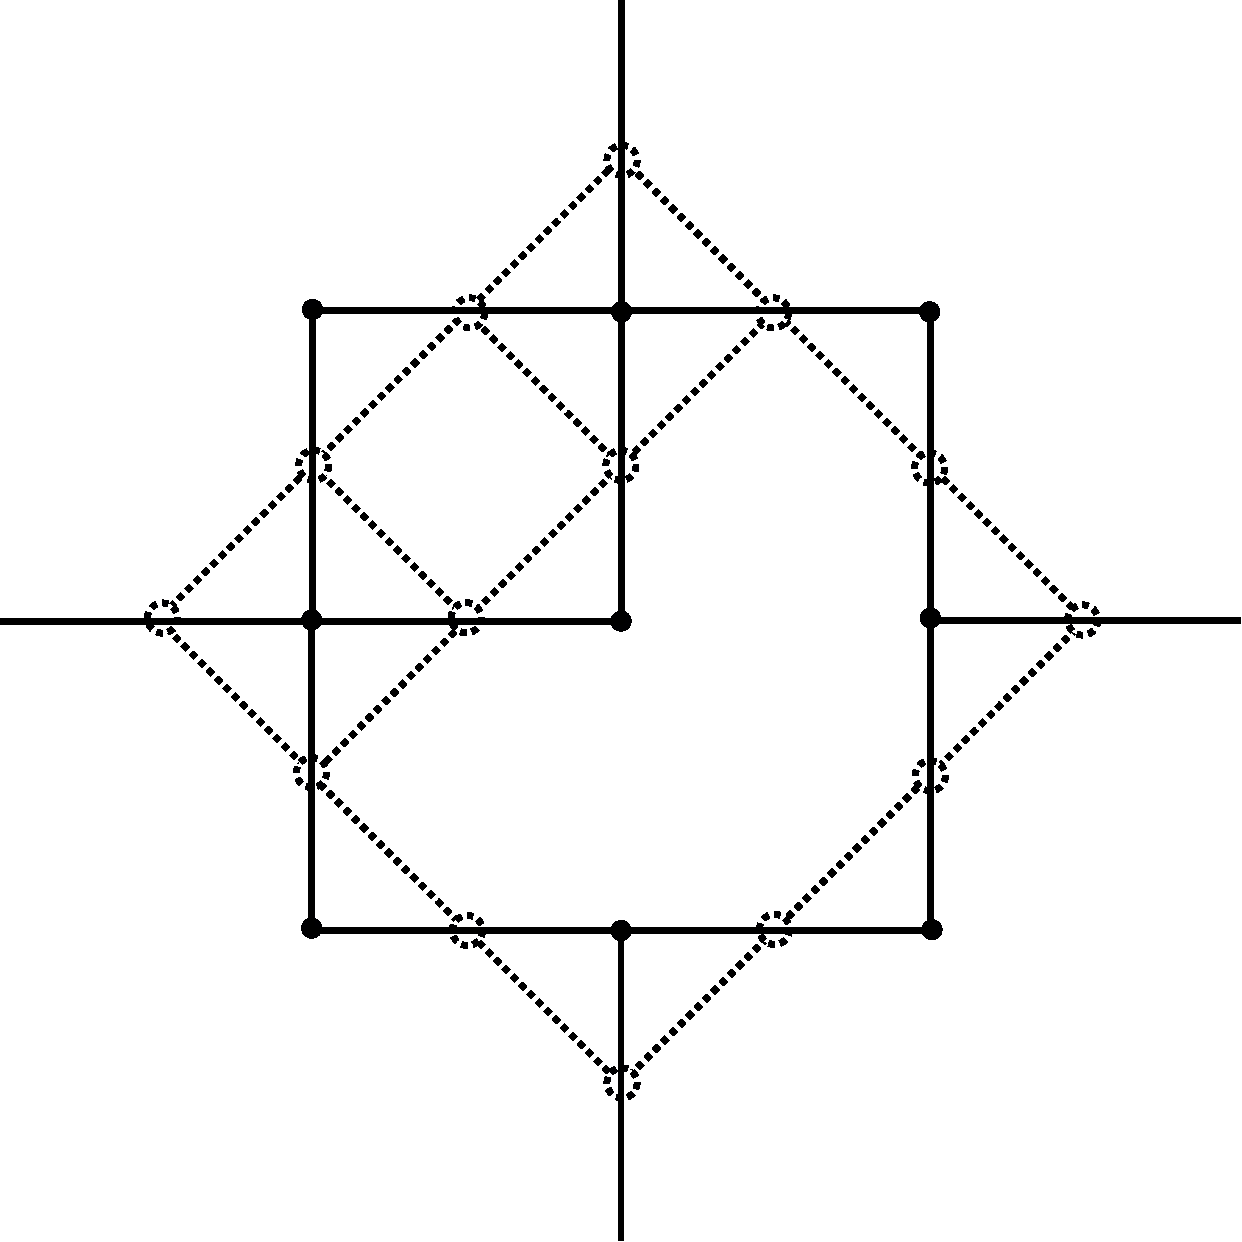
\includegraphics[scale=0.40]{Grid_to_USPIGNC_Fig_2_crop}
  \caption{\label{fig:Grid_to_USPIGNC} Square grid graph $G$ (left).
    Dotted black graph (right) is the intersection graph of axis aligned unit line segments (black) intersecting at end points.
  }
\end{figure}
We now show that HUSPEPIG can be reduced to 3dPP. 
Let each unit line segment be represented by a square block (Figure \ref{fig:Segment_to_Blocka}), which is the union of $9$ unit squares each representing the extruder.
Let the $9$-cluster $C$ be the dual graph of such a square block, consisting of $9$ vertices. % (Figure \ref{fig:Segment_to_Blocka}).
With unit line segments represented by square blocks, there are $3$ types of intersection (Figures \ref{fig:Segment_to_Blockb}, \ref{fig:Segment_to_Blockc}, and \ref{fig:Segment_to_Blockd}).
Each $C$ has four corner vertices.
We can clearly find a Hamiltonian path that starts and ends at distinct corner vertices in $C$ (Figure \ref{fig:Turn_Cost}).
If the start and end vertices are on same side of $C$, then turn cost is $5$, else it is $4$.
We refer to these two traversals of $C$ as type-$1$ and type-$2$, respectively, and incur additional turn costs of $1$ and $0$ for entering and exiting $C$.

Figure \ref{fig:proofoutline} shows the outline of the argument.
We start with the set of axis parallel unit segments (Figure \ref{fig:proofoutlinea}), and its corresponding perpendicular intersection graph $G$ (Figure \ref{fig:proofoutlineb}) with its Hamiltonian cycle (in bold).
Assume without loss of generality that $G$ is connected and has $n>1$ vertices.
We replace unit line segments with square blocks (Figure \ref{fig:proofoutlinec}), which provides the connected polygonal region $R$.
Figure \ref{fig:proofoutlined} shows square blocks replaced by corresponding clusters, and Figure \ref{fig:proofoutlinee} shows 3d printing tour to cover $R$.


\begin{figure}[htp!] 
  \centering
  \begin{subfigure}[t]{2.5in}
    \centering
    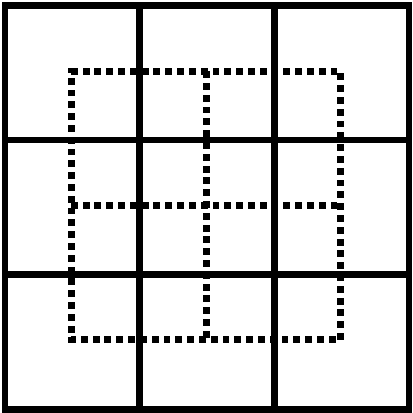
\includegraphics[scale=0.30]{Segment_to_Block_Fig_1_crop}
    \caption{\label{fig:Segment_to_Blocka}}
  \end{subfigure}
  \begin{subfigure}[t]{2.5in}
    \centering
    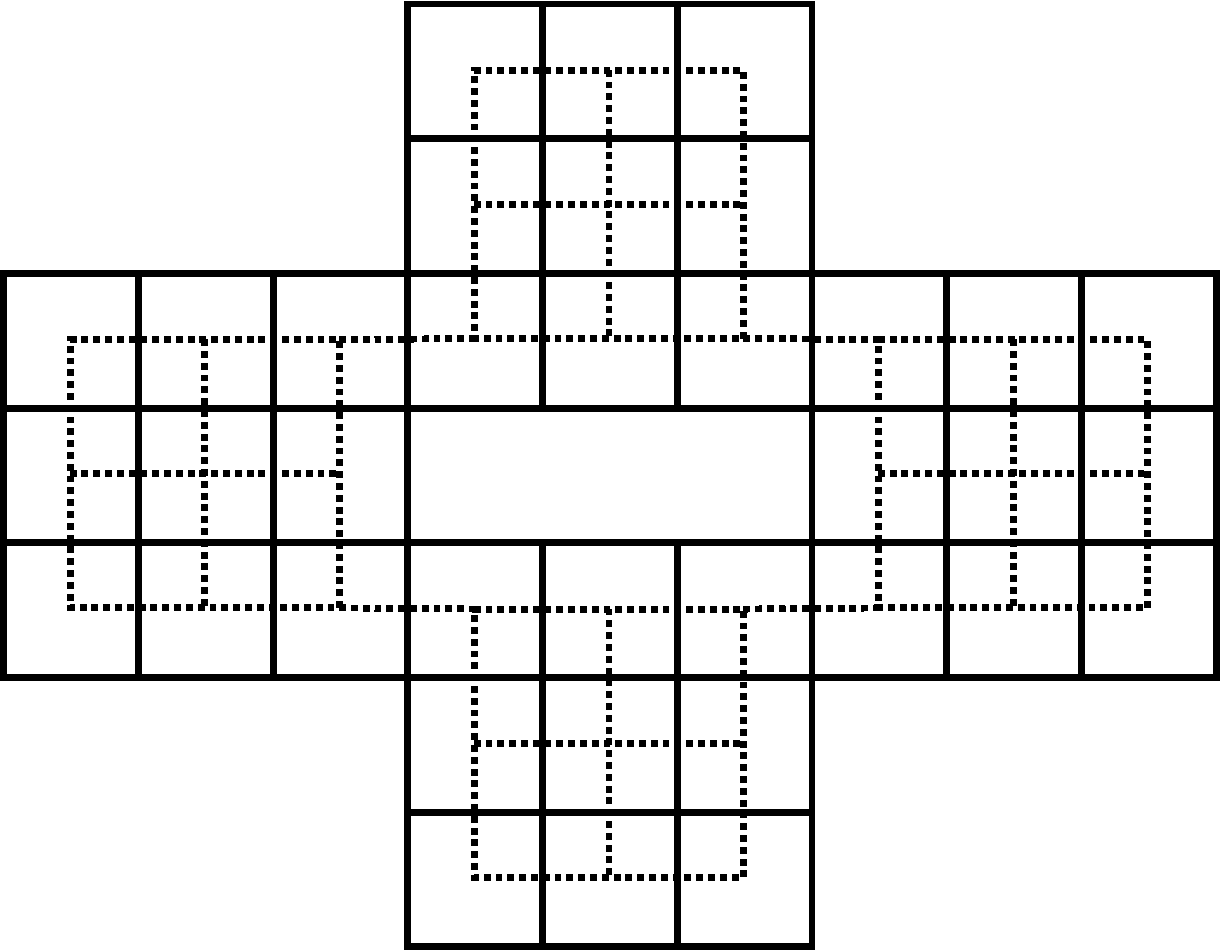
\includegraphics[scale=0.30]{Segment_to_Block_Fig_2_crop}
    \caption{\label{fig:Segment_to_Blockb}}
  \end{subfigure}	
  \begin{subfigure}[t]{2.5in}
    \centering
    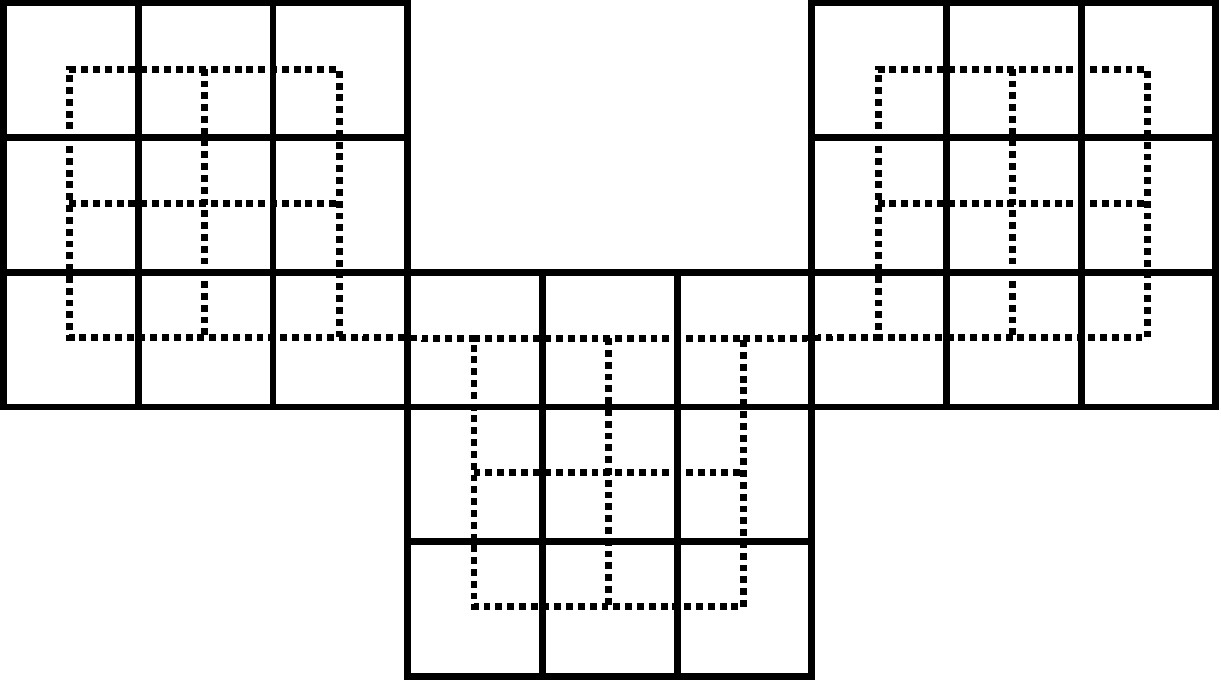
\includegraphics[scale=0.30]{Segment_to_Block_Fig_3_crop}
    \caption{\label{fig:Segment_to_Blockc}}
  \end{subfigure}
  \begin{subfigure}[t]{2.5in}
    \centering
    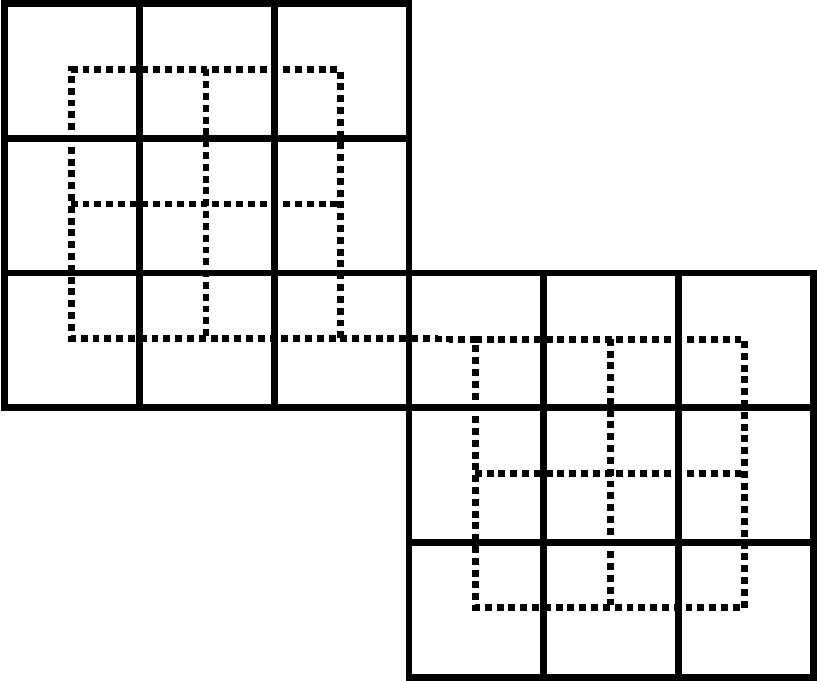
\includegraphics[scale=0.30]{Segment_to_Block_Fig_4_crop}
    \caption{\label{fig:Segment_to_Blockd}}
  \end{subfigure}
  \caption{\label{fig:Segment_to_Block}
    Figure (a): Each unit line segment is represented by a Square Block (solid black) and dual of the Square Block, i.e., its $9$-cluster (dotted black).
    Figures (b), (c), (d): Connectivity based on corresponding unit line segment intersection shown in Figure \ref{fig:USPIGNC_grapha}, \ref{fig:USPIGNC_graphb}, and \ref{fig:USPIGNC_graphc}.
  }
\end{figure}


\begin{figure}[htp!] 
  \centering
  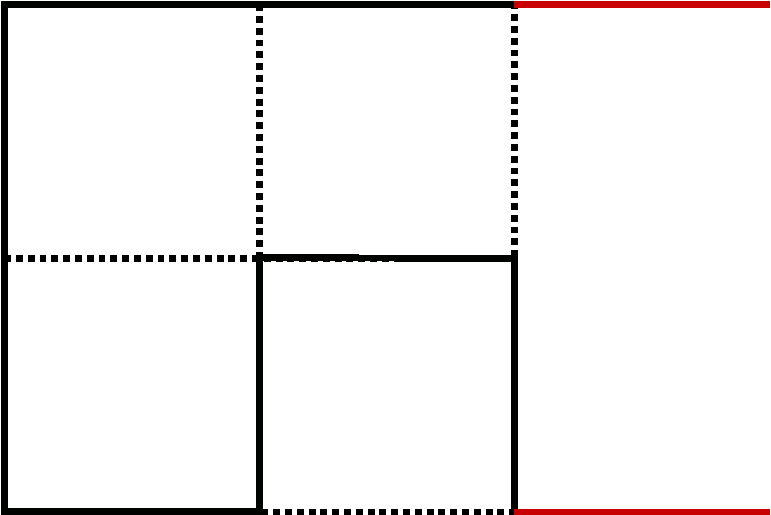
\includegraphics[scale=0.25]{Turn_Cost_Fig_1_crop}
  \hspace*{0.04in}
  %\quad
  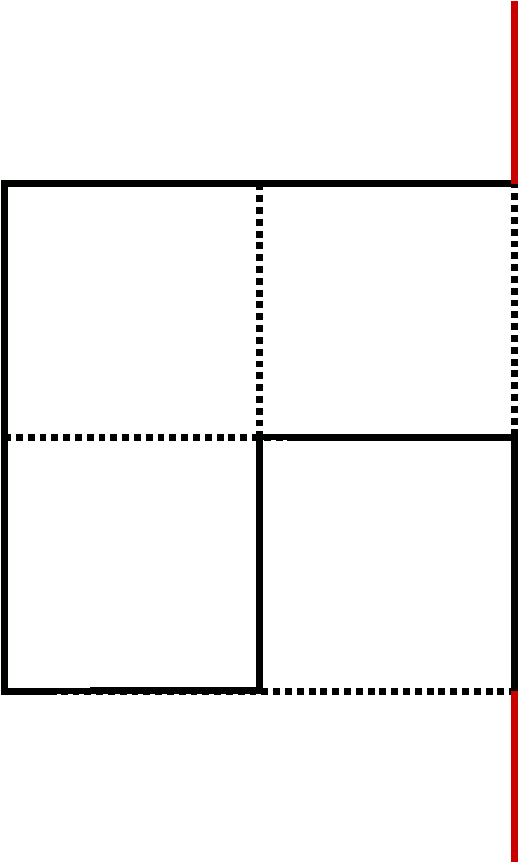
\includegraphics[scale=0.25]{Turn_Cost_Fig_6_crop}
  \hspace*{0.04in}
  %\quad
  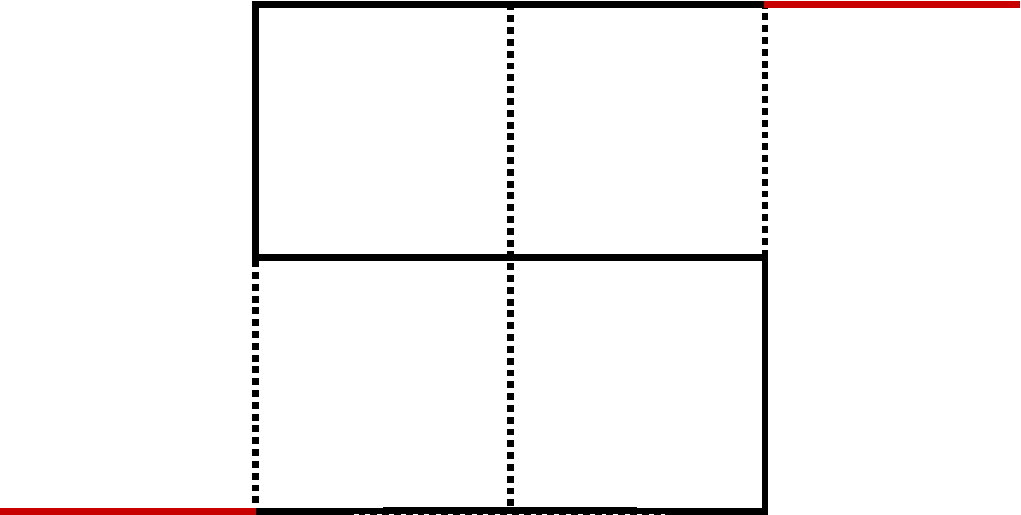
\includegraphics[scale=0.25]{Turn_Cost_Fig_2_crop}
  \caption{\label{fig:Turn_Cost}
    Left and Middle: Hamiltonian path (solid black) with start and end vertices on same side of $C_9$ with turns cost $5$.
    Total entry and exit (red) turn cost for $C_9$ is $1$.
    Right: Hamiltonian path (solid black) with start and end vertices at diagonally opposite corners of $C_9$, with turn cost $4$.
    Total entry and exit (red) turn cost for $C_9$ is $0$.
  }
\end{figure}

\begin{lem}\label{lem:sqblfirt}
  Any Hamiltonian tour of $R$ covers every $9$-cluster $C$ by a single path within $C$.  
\end{lem}

\begin{proof}
  A Hamiltonian tour $H$ of $R$ enters and exits any $9$-cluster $C$ through corner vertices.
  We have two distinct pairs of entry--exit vertices in $C$ for $H$ (as we have four corner vertices).
  Hence we can have at most two paths $p, p'$ within $C$ that are part of $H$.
  Further, since $H$ is a Hamiltonian tour, $p \cap p' = \emptyset$. 

  We consider two possible ways in which $p$ enters and exits $C$.
  First, let $p$ enter and exit at diagonal corner vertices of $C$, e.g., at $a, d$ partially covering $C$ (Figure \ref{fig:lemma33}).
  Since $p$ does not contain $b$ and $c$, and since $p \cap p' = \emptyset$, $p'$ cannot cover all remaining vertices of $C$ without intersecting $p$.
  One such case is shown in Figure \ref{fig:lemma33a}.
  This contradicts the Hamiltonicity of $H$.
  A similar argument holds when $p$ used $b$ and $c$ as end points. 

  Second, let $p$ enter and exit along the same side of $C$, e.g., using $a$ and $b$ (Figure \ref{fig:lemma33b}).
  Then $p'$ with end points $c, d$ cannot cover rest of the vertices of $C$ without intersecting $p$, raising a contradiction.
  %A similar we can show for path $p$ with other pair of end points along the same side.
\end{proof}

\begin{figure}[htp!] 
  \centering
  \begin{subfigure}[t]{2.5in}
    \centering
    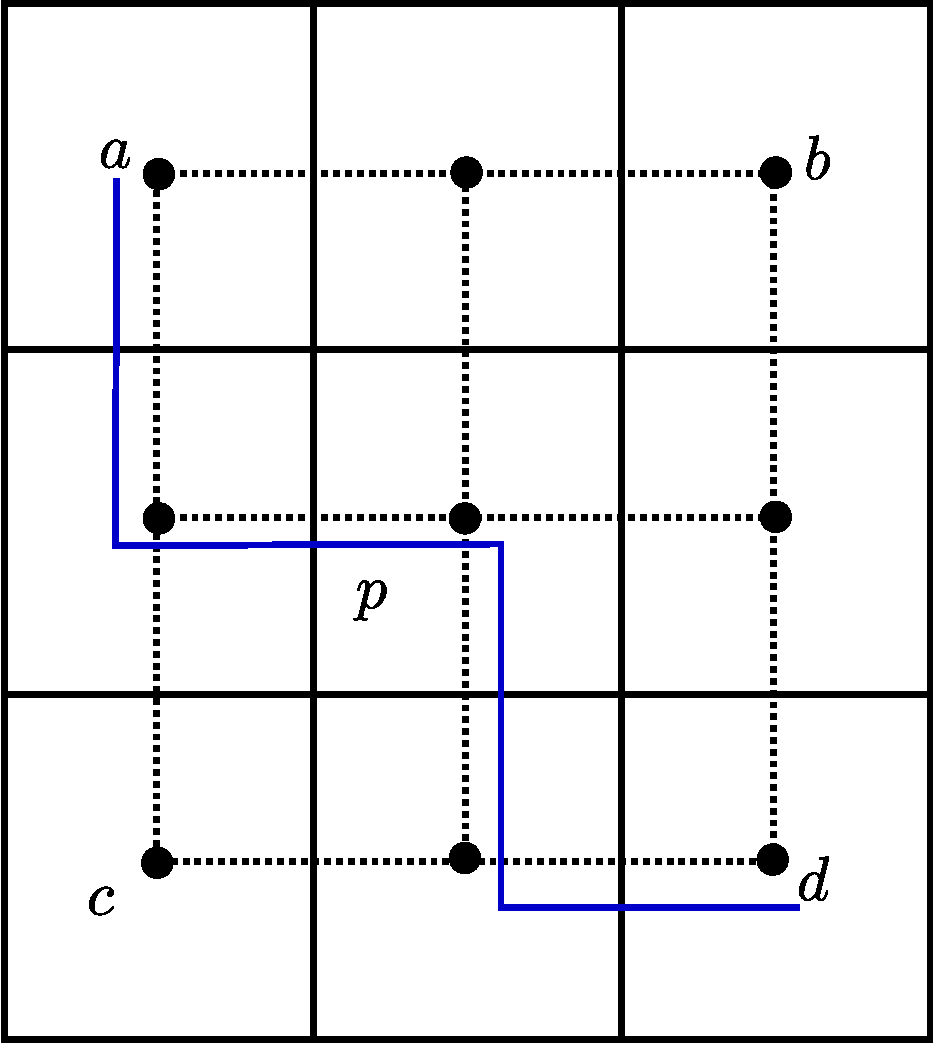
\includegraphics[scale=0.35]{lemma_33_Fig_1_crop}
    \caption{\label{fig:lemma33a}}
  \end{subfigure}
  \begin{subfigure}[t]{2.5in}
    \centering
    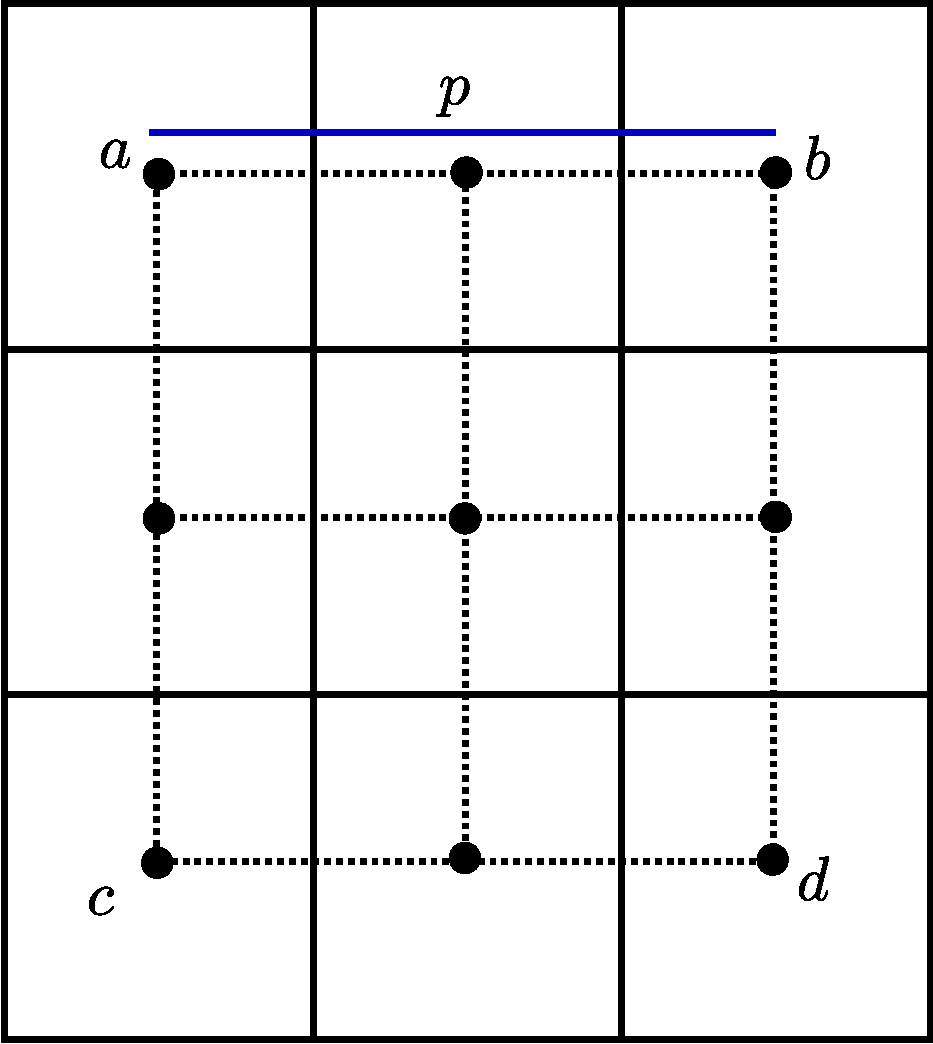
\includegraphics[scale=0.35]{lemma_33_Fig_2_crop}
    \caption{\label{fig:lemma33b}}
  \end{subfigure}	
  \caption{\label{fig:lemma33}
    Proof of Lemma \ref{lem:sqblfirt}.
  }
\end{figure}

\begin{lem}\label{lem:mtpnphard} 
  Minimum Turn 3dPP is NP-hard for any connected polygon $R$ with holes for axis-aligned unit square extruder. 	
\end{lem}
\begin{proof}
  Assume there exists a Hamiltonian tour $H$ in $G$.
  Any move in $H$ from vertex $v_i$ to $v_j$ is equivalent to moving from $9$-cluster $C_i$ to $C_j$ in $R$ by construction.
  By Lemma \ref{lem:sqblfirt}, $H$ covers each $9$-cluster $C_i$ by a single path within $C_i$.
  Further, $H$ uniquely determines the type of traversal (type $1$ or $2$) for each $9$-cluster $C_i$, and hence the numbers $t_1, t_2$ of these clusters such that $t_1 + t_2 = n$.
  This gives a 3dPP tour of $R$  with total turn cost $6t_1+4t_2$ (Figure \ref{fig:Turn_Cost}).

  Conversely, assume there is a 3dPP tour $T$ with turn cost $6t_1+4t_2$ for $t_1, t_2$ being the numbers of type-$1$ and type-$2$ traversals, and $t_1 + t_2 = n$.
  %Let the turn sequence be $u_1, \dots, u_{6t_1+4t_2}$.
  Since $T$ enters and exits each $9$-cluster exactly once (Lemma \ref{lem:sqblfirt}), we are guaranteed a tour of length $n$ in $G$ where each node is traversed exactly once.
  Thus $G$ has a Hamiltonian tour. 	
\end{proof}

\begin{figure*}[htp!] 
  \centering
  \begin{subfigure}[t]{2.5in}
    \centering
    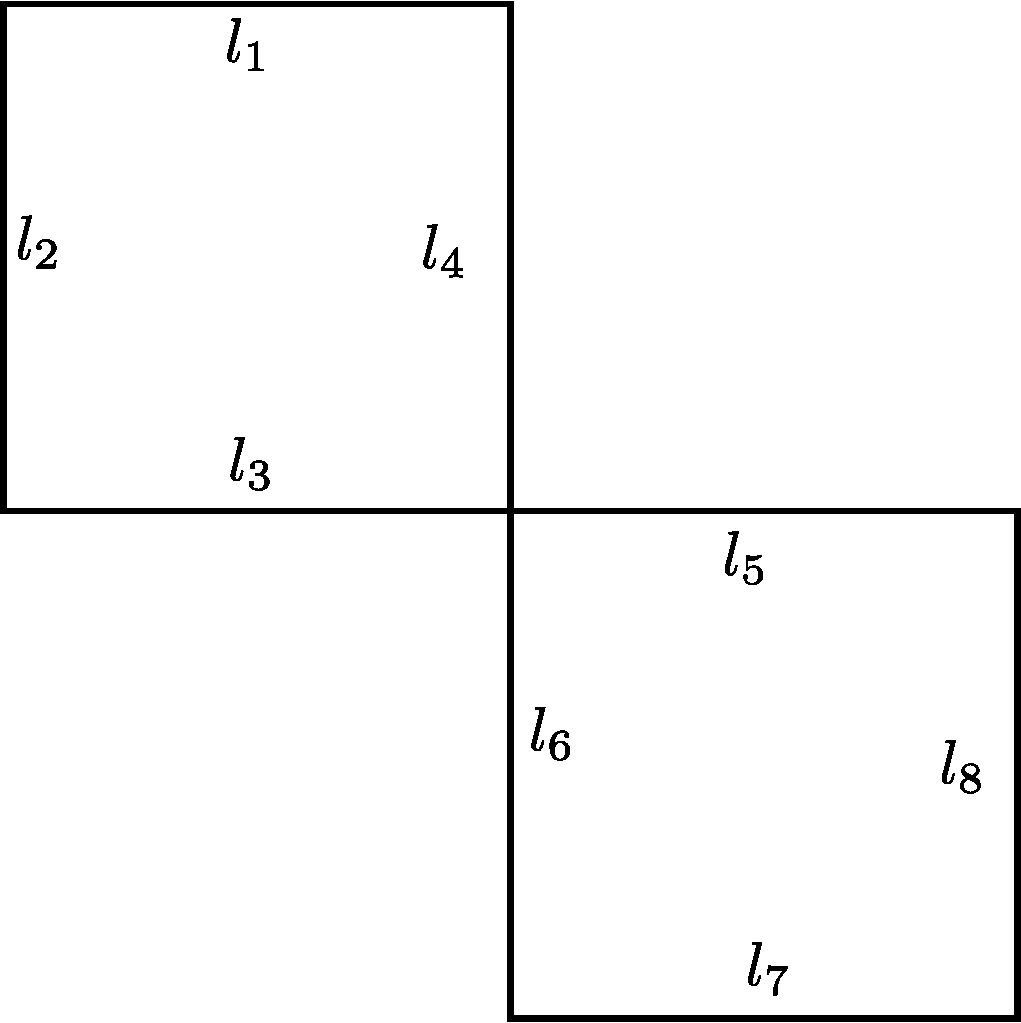
\includegraphics[scale=0.32]{proof_outline_Fig_1_crop}
    \caption{\label{fig:proofoutlinea}}
  \end{subfigure}
  \begin{subfigure}[t]{2.5in}
    \centering
    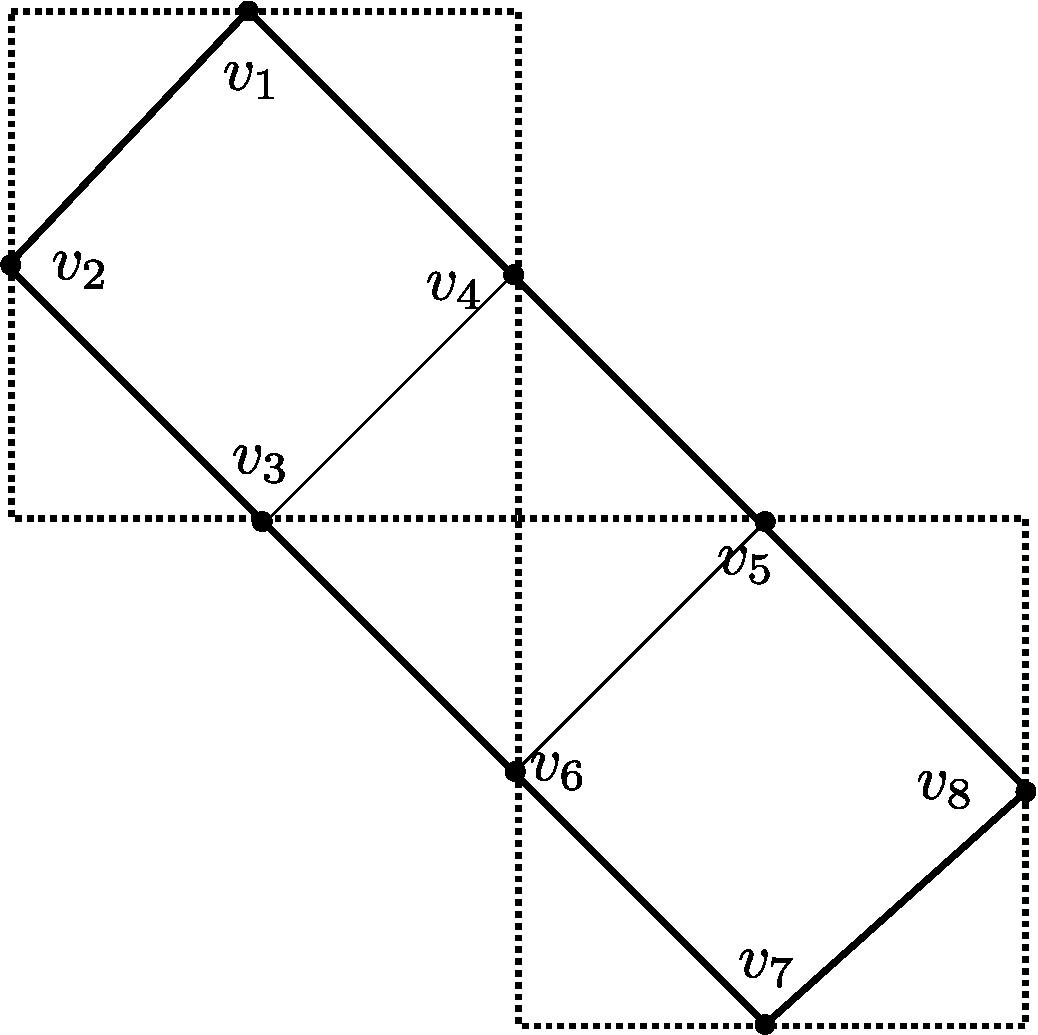
\includegraphics[scale=0.32]{proof_outline_Fig_2_crop}
    \caption{\label{fig:proofoutlineb}}
  \end{subfigure}	
  \begin{subfigure}[t]{2.5in}
    \centering
    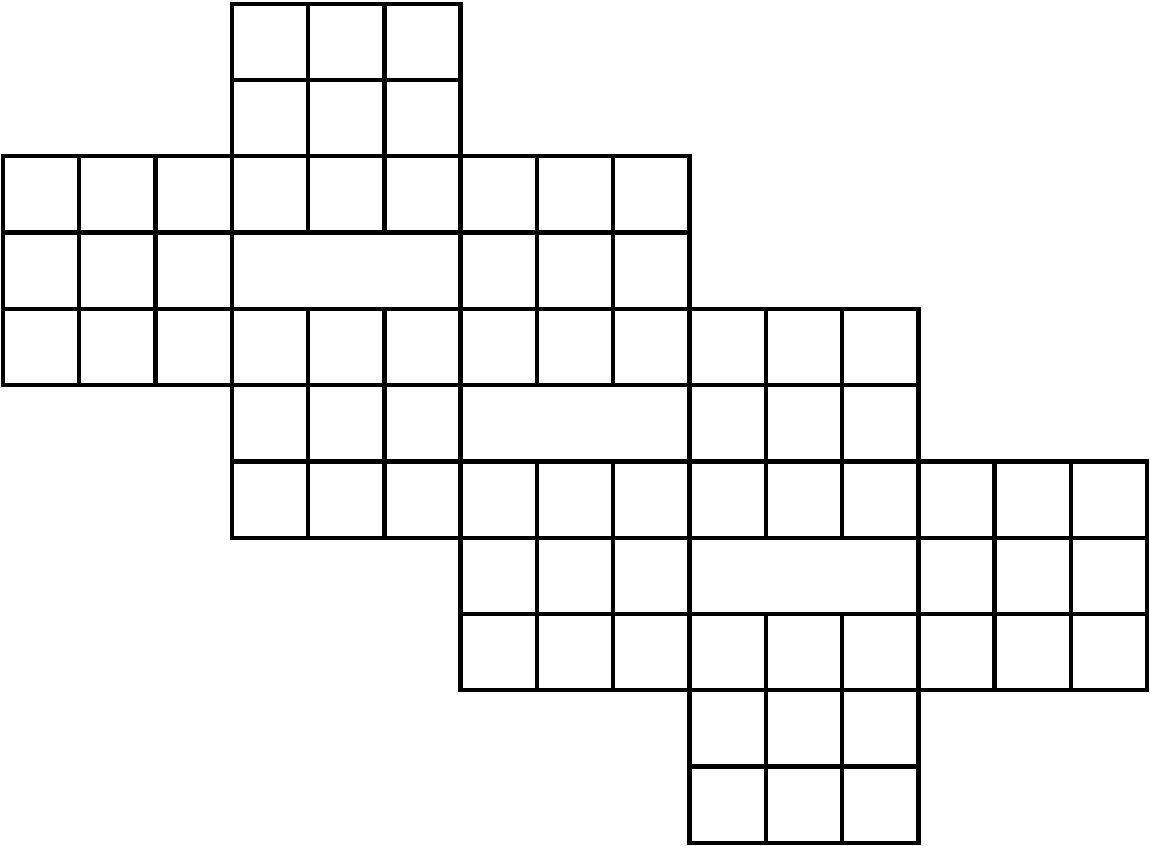
\includegraphics[scale=0.32]{proof_outline_Fig_3_crop}
    \caption{\label{fig:proofoutlinec}}
  \end{subfigure}
  \begin{subfigure}[t]{2.5in}
    \centering
    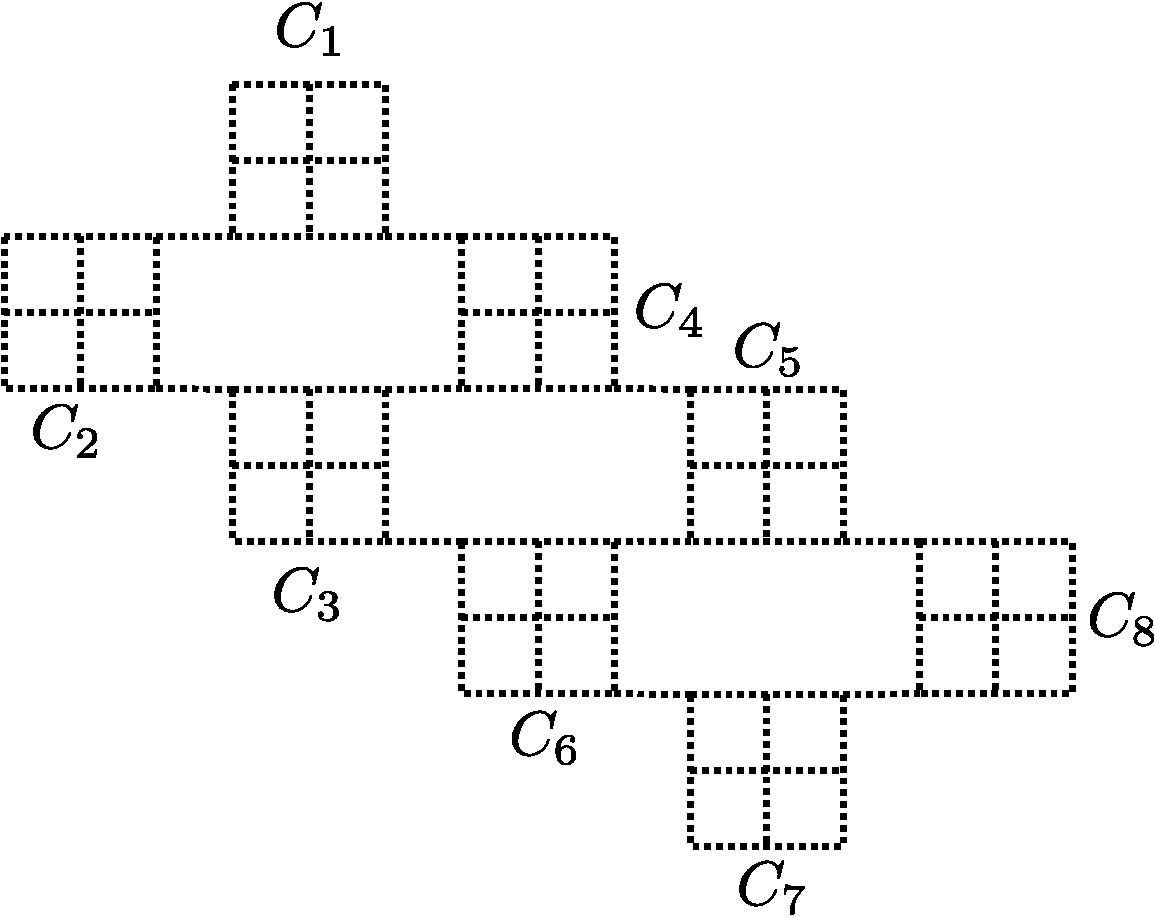
\includegraphics[scale=0.32]{proof_outline_Fig_4_crop}
    \caption{\label{fig:proofoutlined}}
  \end{subfigure}
  \begin{subfigure}[t]{2.5in}
    \centering
    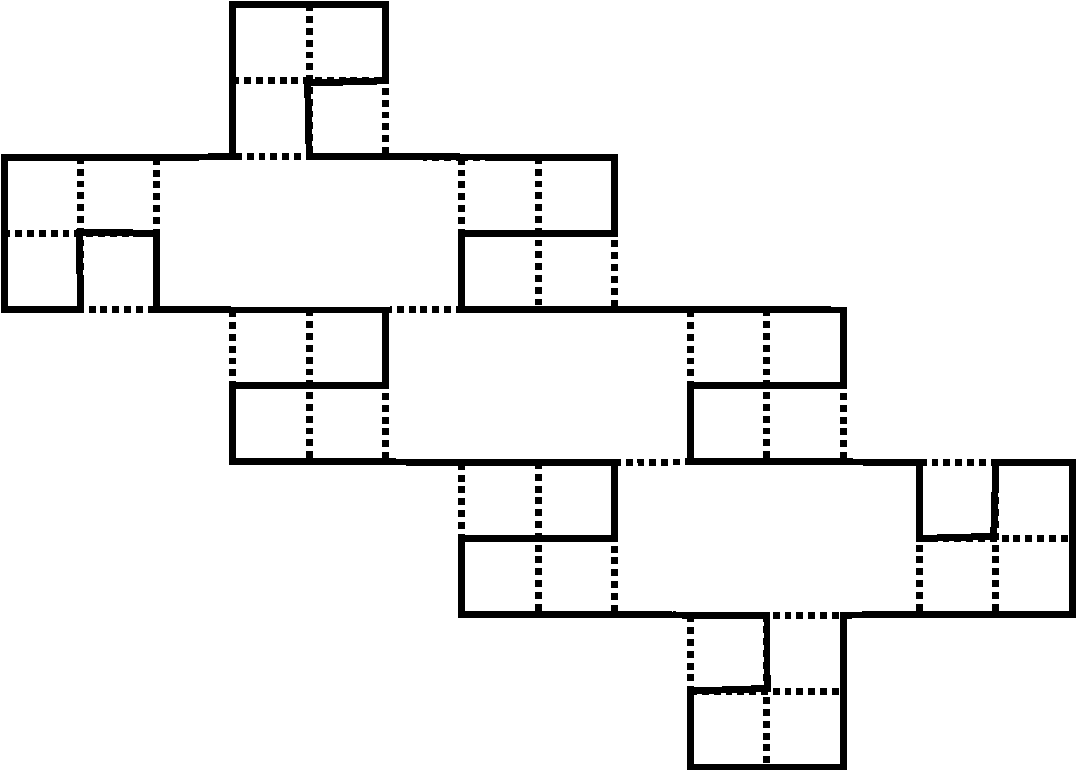
\includegraphics[scale=0.32]{proof_outline_Fig_5_crop}
    \caption{\label{fig:proofoutlinee}}
  \end{subfigure}
  \begin{subfigure}[t]{2.5in}
    \centering
    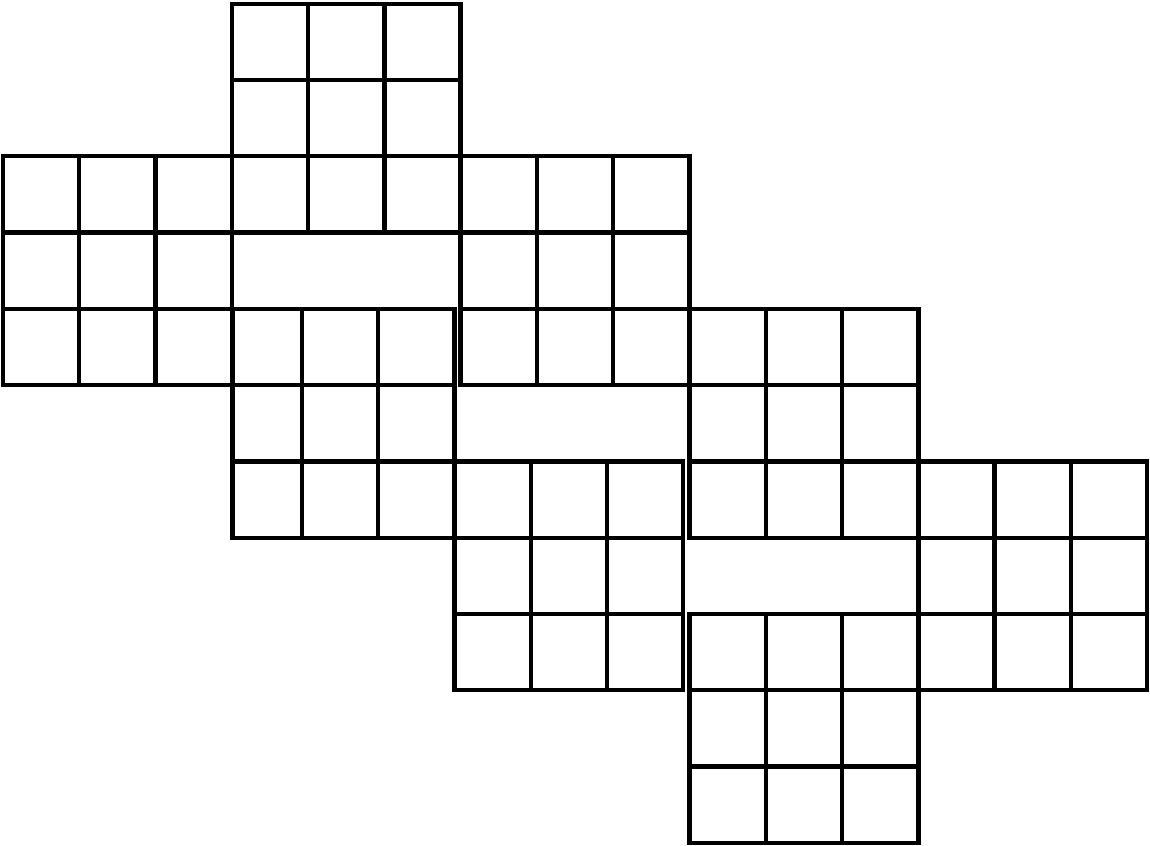
\includegraphics[scale=0.32]{proof_outline_Fig_6_crop}
    \caption{\label{fig:Square_Block_First_Simply_Connected}}
  \end{subfigure}
  \caption{\label{fig:proofoutline}
    See text above Lemma \ref{lem:sqblfirt} for details on Figures (\ref{fig:proofoutlinea})--(\ref{fig:proofoutlinee}).
    Proof of Corollary \ref{cor:nphardsplpoly} is illustrated in Figure (\ref{fig:Square_Block_First_Simply_Connected}).
  }
\end{figure*}

\begin{cor} \label{cor:nphardsplpoly}
  Minimum Turn 3dPP is NP-hard for any simple polygon $R'$ for axis-aligned unit square extruder.
\end{cor}
\begin{proof}
  $R$ in lemma \ref{lem:mtpnphard} can be modified to a simple polygonal region $R'$ by adding narrow slits to connect holes in $R$ (Figure \ref{fig:Square_Block_First_Simply_Connected}).
  Let the width of each slit be $w/n'$ for $n' \geq n$ and $w \leq 1$.
  Addition of slits does not add any turn cost, since it is the same 3dPP with {\it total} idle movement $n(w/n') = \epsilon \leq 1$. 
  By Lemma \ref{lem:mtpnphard}, a Hamiltonian tour of length $n$ on $G$ gives a 3dPP tour with turn cost $6t_1 + 4t_2 $ for $R$. 
  This implies there is a 3dPP tour with turn cost $6t_1 + 4t_2$ on $R'$, since total idle movement is less than equal to $1$.
  Conversely, let $R'$ have a tour with turn cost $6t_1 + 4t_2$.
  Then total turn cost of a tour in $R$ is also $6t_1 + 4t_2$, since idle movement in $R'$ is $\leq 1$. 
  Hence it corresponds to a Hamiltonian tour of length $n = t_1 + t_2$ in $G$ by Lemma \ref{lem:mtpnphard}.
\end{proof}
\section{Traversal} \label{sec:travseral}

We use a {\it quadtree} structure to decompose the integral orthogonal polygon (IOP) $P$ into square cells.
Then we join some of the square cells to create bigger cells.
We then identify the traversal order of these cells using a Hilbert space filling curve.
Our decomposition approach will work also with other rectilinear space filling curves such as Peano or Moore curves.
\subsection{Quadtree}\label{ssec:quadtree}
The quadtree decomposition of IOP $P$ is created as follows.
\textit{First}, find the smallest initial cell $[0, 2^m] \times [0, 2^m]$ that contains $P$, where $m>0$ is an integer.
\textit{Second}, apply adaptive subdivision of initial cell until all cells are completely inside or outside of $P$.
Remove cells completely outside of $P$ from the quadtree.
\textit{Third}, further subdivide cells if area of any cell is more than $\delta > 0$, an integer.
An example of quadtree is shown in the Figure \ref{fig:quadtree_example_combine}.

We want to ensure that each leaf cell in the quadtree is traversed at least once by the toolpath algorithm.
One way is to do depth first traversal, where we recursively follow the left most unvisited branch until we reach a leaf cell.
Once done with leaf cell, backtrack until the first cell which has a left most unvisited child cell, and so on.
This gives us a sequential ordering of cells (see example in Figure \ref{fig:quadtree_example_combinec}).
But jumps could be pretty large between neighboring cells in this sequence.
Instead, we create a sequence based on a Hilbert ordering such that neighboring cells are also adjacent (see Figure \ref{fig:quadtree_example_combined}).

\begin{figure}[htp!] 
  \centering
  \begin{subfigure}[t]{2.5in}
    %\centering
    \hspace*{-0.15in}
    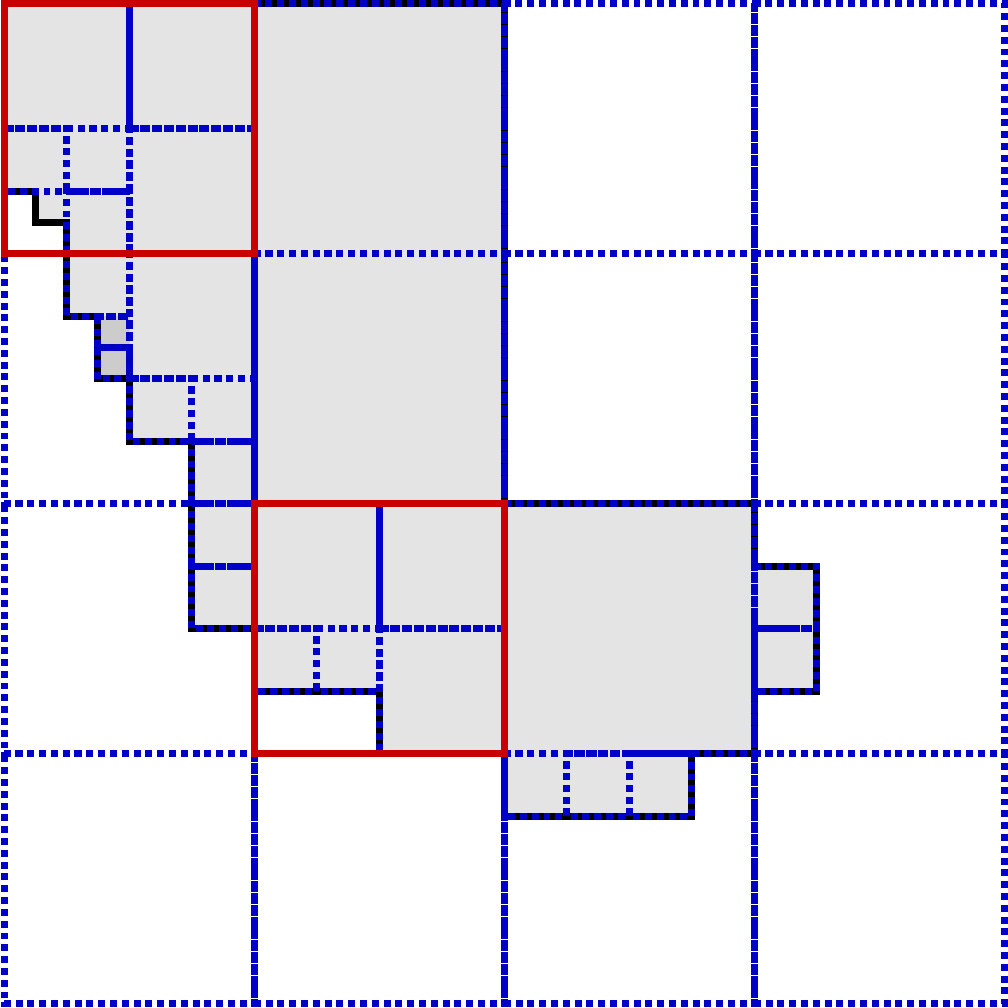
\includegraphics[scale=0.35]{quadtree_Example_Figure_2_crop}
    \caption{\label{fig:quadtree_example_combinea}}
    \medskip
  \end{subfigure}
  \begin{subfigure}[t]{2.5in}
    %\centering
    \hspace*{-0.1in}
    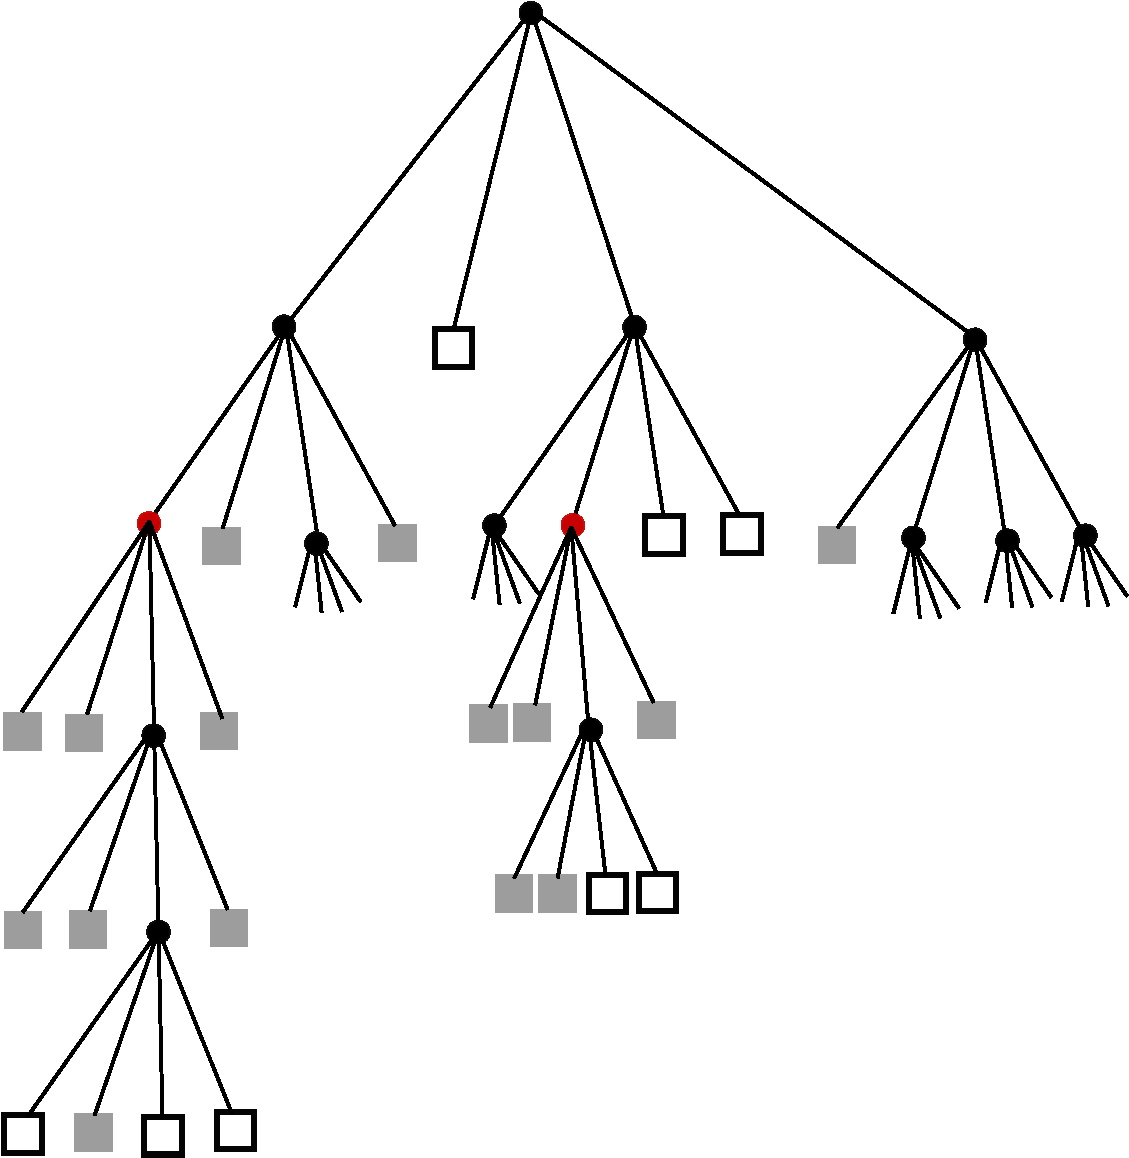
\includegraphics[scale=0.35]{quadtree_Example_Figure_4_crop}
    \caption{\label{fig:quadtree_example_combineb}}
    \medskip
  \end{subfigure}
  \begin{subfigure}[t]{2.5in}
    %\centering
    \hspace*{-0.15in}
    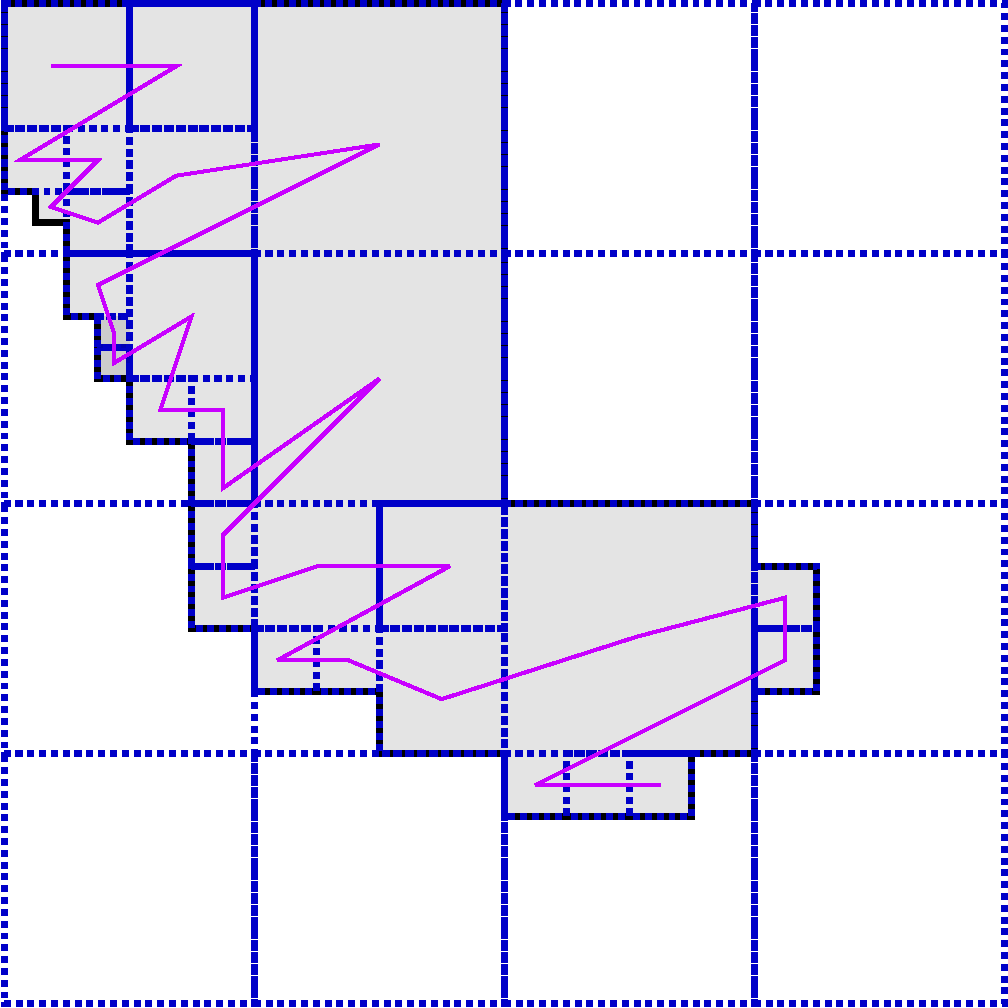
\includegraphics[scale=0.35]{quadtree_Example_Figure_5_crop}
    \caption{\label{fig:quadtree_example_combinec}}
  \end{subfigure}
  \begin{subfigure}[t]{2.5in}
    \centering
    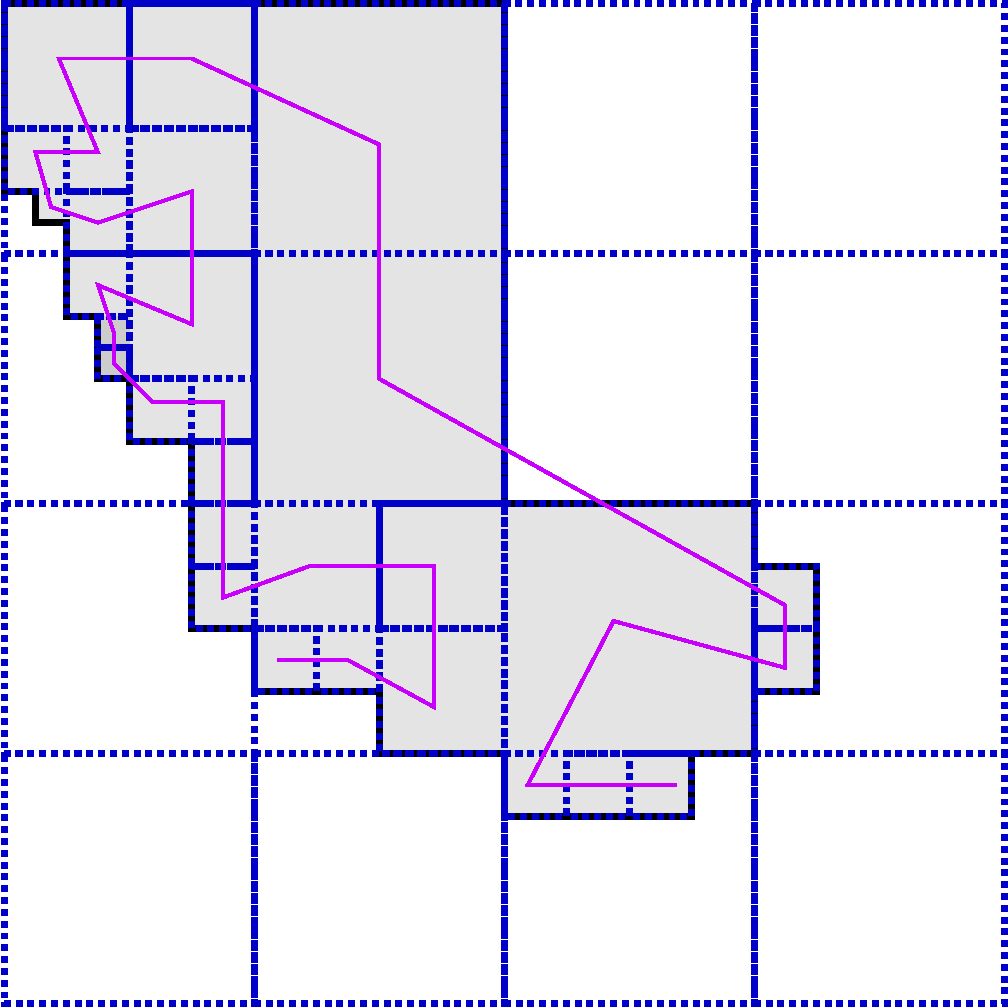
\includegraphics[scale=0.35]{quadtree_Example_Figure_6_crop}
    \caption{\label{fig:quadtree_example_combined}}
  \end{subfigure}
  \medskip
  \caption{\label{fig:quadtree_example_combine}
    In Figure (\ref{fig:quadtree_example_combinea}), red cells will be further subdivided since they are not completely inside the polygon.
    Figure (\ref{fig:quadtree_example_combineb}) shows the quadtree where red nodes represents red cells in Figure (\ref{fig:quadtree_example_combinea}) further subdivided, shaded square nodes represent cells completely inside polygon, and empty square nodes represent cells completely outside polygon and will be removed from the tree.
    Figures (\ref{fig:quadtree_example_combinec}) and (\ref{fig:quadtree_example_combined}) show sequential ordering of leaf node cells using depth first traversal and Hilbert ordering.
  }  	
\end{figure}
\subsection{Ordering and Properties of Square Cells} \label{ssec:squarecells}

For illustration, consider an $8 \times 8$ square domain and its $2 \times 2$ cells generated from subdivision using quadtree with $\delta = 4$, and Hilbert ordering of its cells as shown in Figure \ref{fig:celltour}.
To generate a Hilbert curve we need to identify entry and exit corners for each cell.
Suppose the Hilbert curve enters at $(0, 0)$ and exits at $(8, 0)$.
Due to its properties, the Hilbert curve will enter and exit the cell at points that are along an edge of the cell (and not diagonally opposite), as shown in Figure \ref{fig:celltoura}.
Each cell $C$ (from now on, we refer to these cells as $C$ or $C_i$) in Figure \ref{fig:celltoura} is a union of pixels, as they are square with integer length.
Let $G$ be the dual graph of pixel graph of cell $C$, and let entry ($s$) and exit ($t$) vertices in $G$ be the vertices closest to the Hilbert curve in $C$.
We ensure all the vertices in the dual graph of the pixel graph of cell $C$ are covered in the following way.
{\bfseries \textit{First}}, find the path for each $G$ using the IP model in Section \ref{sec:ipmodel} for a given choice of entry ($s$) and exit ($t$) vertices (Figure \ref{fig:celltourb}).
{\bfseries \textit{Second}}, join these paths by a connecting path between exit and entry vertices of neighboring graphs in corresponding cells' Hilbert ordering (Figure \ref{fig:celltourc}).
If length of the connecting path is more than one unit, then it is set as idle movement of the extruder.
 
Note that the traversal of IOP can be a walk due to idle movements of the extruder.
We call a finite sequence of vertices and edges where both vertices and edges can be repeated a {\em walk}, and a {\it path} when vertices and edges are not repeated. 
\begin{figure*}[htp!] 
  \centering
  \begin{subfigure}[t]{1.8in}
    \centering
    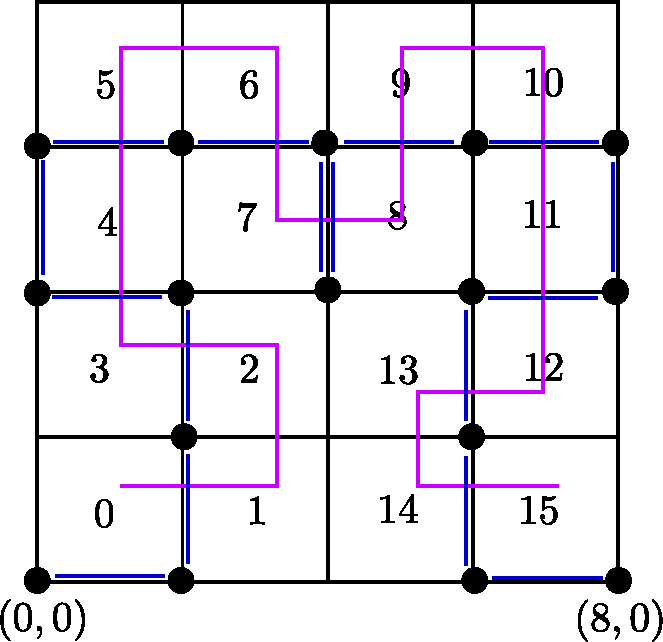
\includegraphics[scale=0.37]{quadtree_Example_Figure_9_crop}
    \caption{\label{fig:celltoura}}
  \end{subfigure}
  \begin{subfigure}[t]{1.8in}
    \centering
    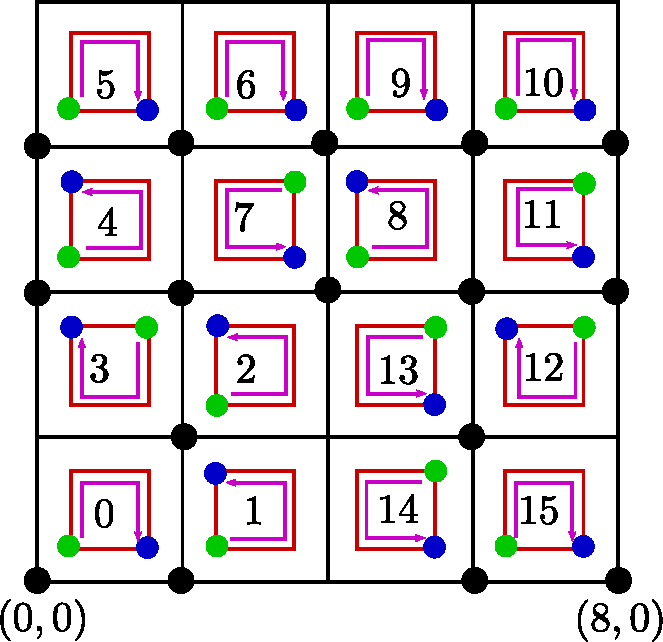
\includegraphics[scale=0.37]{quadtree_Example_Figure_10_crop}
    \caption{\label{fig:celltourb}}
  \end{subfigure}	
  \begin{subfigure}[t]{1.8in}
    \centering
    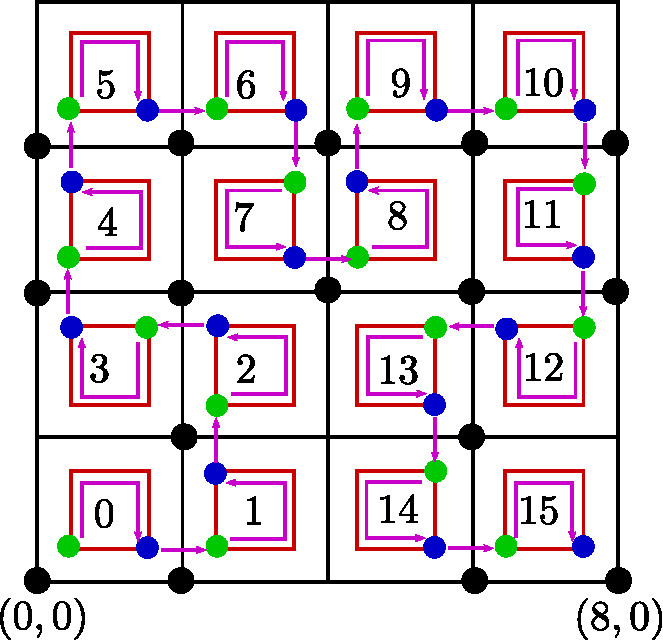
\includegraphics[scale=0.37]{quadtree_Example_Figure_11_crop}
    \caption{\label{fig:celltourc}}
  \end{subfigure}
  \caption{\label{fig:celltour} Black dots in Figure \ref{fig:celltoura} represent entry and exit vertices for each cell from $0$ to $15$, and Hilbert ordering of the cells is in pink.
    Figure \ref{fig:celltourb} shows entry vertex (green dot) and exit vertex (blue dot) for dual graph (red) of pixel graph of each cell.
    Paths shown in pink covers all vertices of dual graphs.
    Figure \ref{fig:celltourc} shows connecting paths in pink which connect paths on dual graphs based on Hilbert ordering of corresponding cells.} 
\end{figure*}


Entry and exit vertices of any $G$ identified by this approach are corner vertices in $G$ that can be joined by a straight path.
Let $(G, s, t)$ be a Hamiltonian $s$-$t$ path problem for  distinct vertices $s$ and $t$.
We show that $(G, s, t)$ always has a solution.
First we will review certain properties of grid graph.
A grid graph is a finite graph whose vertices are points with integer coordinates, and two vertices are connected if they are unit distance apart.
Let $(v_x, v_y)$ be the coordinates of vertex $v$.
Then $v$ is even if $v_x + v_y = 0 (\mod 2)$, else $v$ is odd.
This implies that grid graphs are bipartite, with edges connecting even and odd vertices.
Let $R(m ,n)$ be the grid graph whose vertex set is $\{v: 1 \leq v_x \leq m, ~ 1\leq v_y \leq n \}$.
Rectangular graph is a grid graph isomorphic to $R(m, n)$.
We review the necessary conditions for existence of a Hamiltonian path in rectangular graphs \cite{ItPaSz1982}.
We also denote $R(m,n)$ by $B = (V^0 \cup V^1, E)$, the bipartite graph.
Since $B$ is two colorable, let all vertices in $V^0$ are of one color and all vertices in $V^1$ are of a second color.

\subsubsection{Solution for the Hamiltonian path problem $(B, s, t)$} \label{list:hamipathexist}
This exists if at least one of the following conditions is {\it not} satisfied. 
\begin{enumerate}
  \item $B$ is even $(|V^0| = |V^1|)$ and $s$ and $t$ are of the same color, or $B$ is odd, say, with $|V^0| = |V^1| + 1$, and $s, t \in V^1$. 
  \item $n = 1$ and either $s$ or $t$ is not a corner vertex (Figure \ref{fig:hamiltonianconda}).
  \item $n = 2$ and edge $st$ is not a boundary edge (Figure \ref{fig:hamiltoniancondb}). 
  \item $n = 3$ and it satisfies following conditions (Figures \ref{fig:hamiltoniancondc}, \ref{fig:hamiltoniancondd}):
    \begin{enumerate}
      \item $s$ is different color from $t$, and $t$ is different color from the top corner vertices; and 
      \item $s_x \leq t_x - 1$ or $(s_y = 2$ and $s_x \leq t_x)$. 
    \end{enumerate}
\end{enumerate}

\begin{figure}[htp!] 
  \centering
  \begin{subfigure}[t]{1in}
    \centering
    
\includegraphics[scale=0.40,angle=270]{hamiltonian_condition_Figure_1_crop}
    \caption{\label{fig:hamiltonianconda}}
  \end{subfigure}
  \begin{subfigure}[t]{1in}
    \centering
    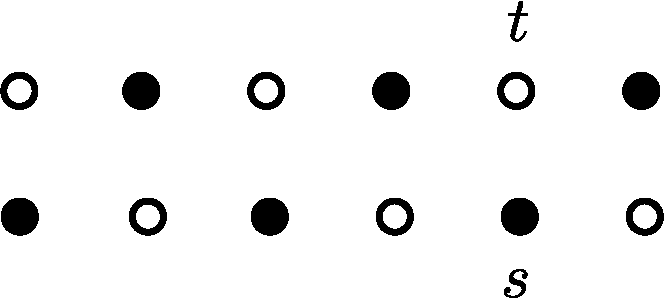
\includegraphics[scale=0.40,angle=270]{hamiltonian_condition_Figure_2_crop}
    \caption{\label{fig:hamiltoniancondb}}
  \end{subfigure}	
  \begin{subfigure}[t]{1.7in}
    \centering
    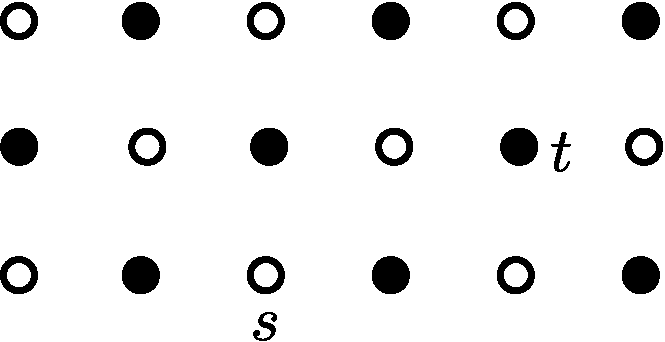
\includegraphics[scale=0.40,angle=270]{hamiltonian_condition_Figure_3_crop}
    \caption{\label{fig:hamiltoniancondc}}
  \end{subfigure}
  \begin{subfigure}[t]{1.7in}
    \centering
    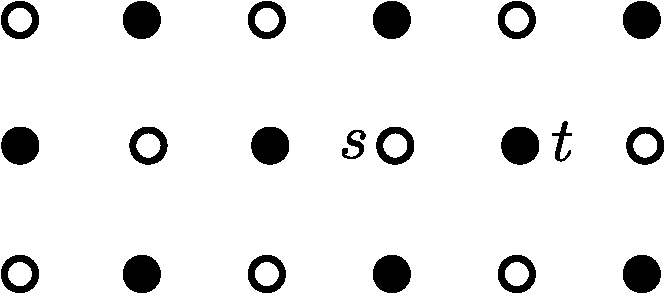
\includegraphics[scale=0.40,angle=270]{hamiltonian_condition_Figure_4_crop}
    \caption{\label{fig:hamiltoniancondd}}
  \end{subfigure}
  \caption{\label{fig:hamiltoniancond}
    Cases that prevent Hamiltonian path problem $(B,s,t)$ from having a solution (Section \ref{list:hamipathexist}).
  }
\end{figure}

\begin{lem}\label{lem:hamiltonianpathexist}
  Let $(G, s, t)$ be a Hamiltonian path problem on $G$, the dual graph of pixel graph of a cell $C$, and $s$ and $t$ are entry and exit vertices of the Hamiltonian path.
  Then $(G, s, t)$ has a solution.
\end{lem}
\begin{proof}
  If area of $C$ is one unit then it is a trivial case, since $G$ has one vertex.
  More generally, the entry and exit vertices $s$ and $t$ are corner vertices in $G$, and are joined by a straight path.
  This straight path has even number of vertices.
  Hence $s$ and $t$ have different colors.
  Further, we have equal number of even and odd vertices in any $G$.
  Hence a Hamiltonian path always exists, as none of the conditions (Section \ref{list:hamipathexist}) is satisfied.   
\end{proof}

\subsection{Join Square Cells}\label{ssec:joincell}

We now try to join some square cells into bigger cells, so that we can solve larger instances of the subproblems to reduce turn costs.
Let $G_i$ be the dual graph corresponding to square cell $C_i$.
Let $S = \{C_1, \dots, C_m\}$ be the sequence of square cells based on Hilbert ordering for an IOP $P$, and $G(S) = \{G_1, \dots, G_m\}$ is the  corresponding sequence of dual graphs.
Let $(G_k, s_k, t_k)$ be the Hamiltonian path problems for $k \in [m] \coloneq \{1, ... , m\}$ and $s_k, t_k$ are chosen as in Section \ref{ssec:squarecells}.
Rectilinear distance between any two ordered neighbors $G_i, G_{i+1}$ in sequence $G(S)$ is defined as $d(G_i,G_{i + 1}) = |t_i^x - s_{i+1}^x| + |t_i^y - s_{i+1}^y|$.

Now we will join square cells as follows.
{\bfseries{\textit{First}}}, let $G(S_i)= \{G_l, \dots, G_{l+k}\}$ where $d(G_{l-1},G_{l}) > 1$ or $l=1$, and $d(G_{l+k},G_{l+k+1})$ $>1$ or $l+k=m$ and $d(G_{i},G_{i+1})= 1 ~\forall i \in \{l, \dots, l+k-1\}$.
Find subsequence set $\{G(S_i)\}$ from $G(S)$.
{\bfseries{\textit{Second}}}, let $\tilde{C}_j$ be union of all the cells in subsequence $\tilde{S}_j$ of $S_i$.
Consider $\tilde{C}_j$ as an IOP.
Partition $S_i$ into a set of subsequences $\{\tilde{S}_j\}$ such that total area of $\tilde{C}_j$ is $\leq \Delta$, where $\Delta$ is maximum area allowed in any $\tilde{S}_j$ (see Figures \ref{fig:quadtreejoina}, \ref{fig:quadtreejoinb}).
%An example is shown in .  

\begin{lem}\label{lem:joinedgraphhamiltonianpathexist}
  Let $\{G_1, \dots, G_m\}$ be a sequence of dual graphs corresponding to sequence $\{C_1, \dots, C_m\}$ whose union is $\tilde{C}_j$, $(G_k, s_k, t_k)$, $(\tilde{G}_i, s, t)$ are Hamiltonian path problems, where $\forall k \in \{1, ... , m\}$ and $s_k, t_k$ $\forall k$ is chosen based on section \ref{ssec:squarecells} and $\tilde{G}_i$ is dual graph of pixel graph of $\tilde{C}_i$.
  If $s= s_1$, $t = t_m$ then $(\tilde{G}_i, s, t)$ has a solution.
\end{lem}
\begin{proof}
  By Lemma \ref{lem:hamiltonianpathexist}, a Hamiltonian path exists $\forall (G_i, s_i, t_i)$.
  The Hamiltonian path from $G_i$ is joined with the one from $G_{i+1}$ by an edge $\{t_i, s_{i+1}\}$ in $\tG_i$, and $s = s_1$, $t = t_m$.
  The result follows.
  %Hence the result follows.
  % $(\tG_i, s, t)$ has a solution.
\end{proof}

\begin{figure}[htp!]
  \medskip
  \centering
  \begin{subfigure}[t]{1.8in}
    %\centering
    %\hspace*{-0.15in}
    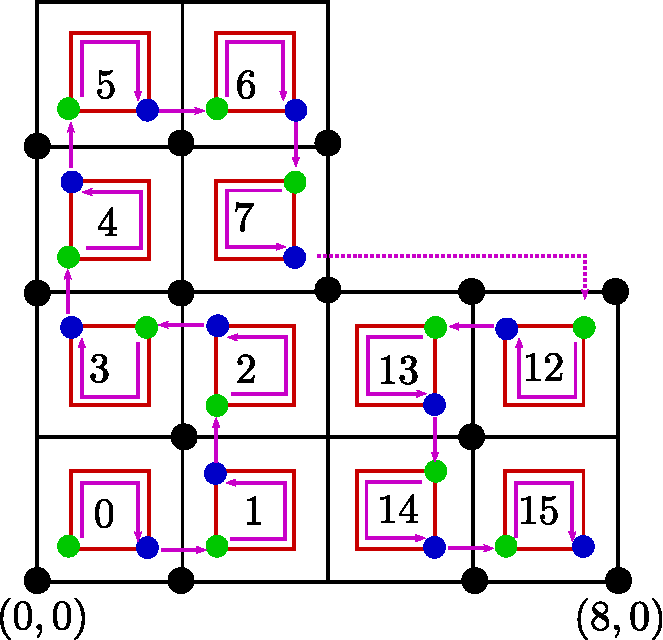
\includegraphics[scale=0.4]{quadtree_join_graph_Fig_0_crop}
    \caption{\label{fig:quadtreejoina}}
  \end{subfigure}
  %\hfill
  \begin{subfigure}[t]{1.8in}
    %\centering
    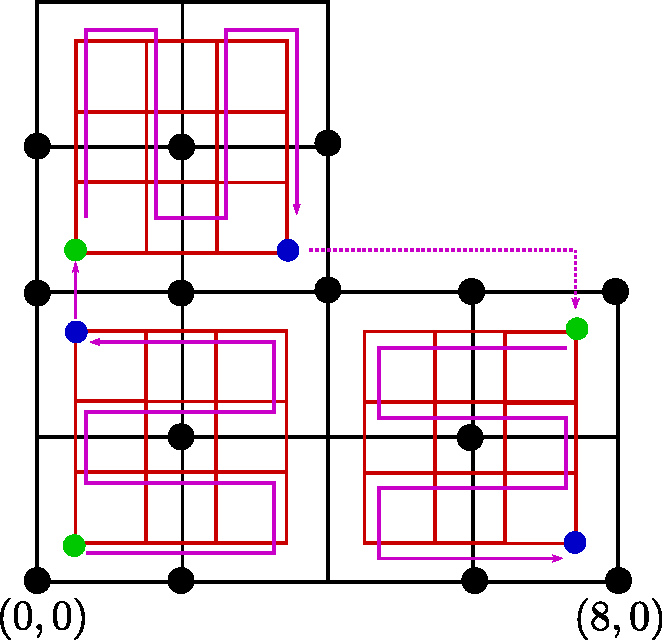
\includegraphics[scale=0.4]{quadtree_join_graph_Fig_1_crop}
    \caption{\label{fig:quadtreejoinb}}
  \end{subfigure}
  \begin{subfigure}[t]{1.8in}
    %\bigskip
    \centering
    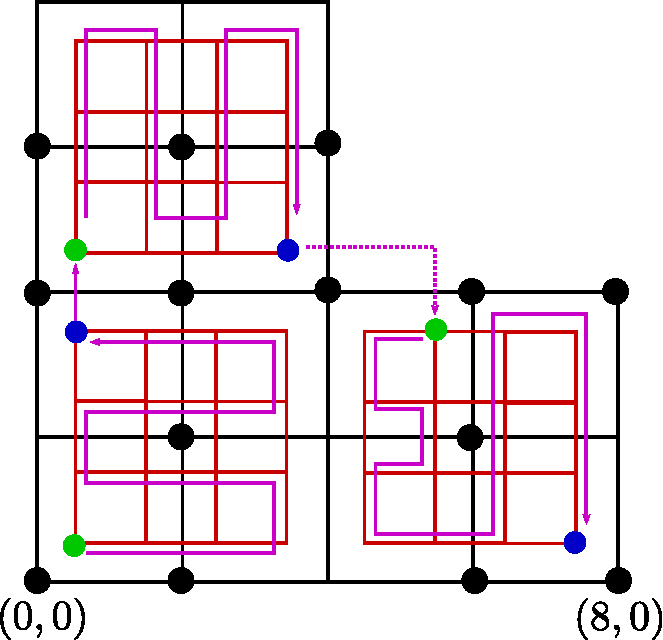
\includegraphics[scale=0.4]{quadtree_update_enter_exit_graph_Fig_1_crop}
    \caption{\label{fig:quadtreejoinc}}
  \end{subfigure}
  \caption{\label{fig:quadtreejoin}
    Path (pink) in Figure \ref{fig:quadtreejoina} covers the IOP.
    Idle movement of path is shown in pink dots.
    Further, Hilbert ordering of the cells is $[0, 1, 2, 3, 4, 5, 6, 7, 12, 13, 14, 15]$.
    Figure \ref{fig:quadtreejoinb} shows $3$ joined square cells based on Hilbert ordering into $[0, 1, 2, 3], [4, 5, 6, 7], [12, 13, 14, 15]$ with $\Delta = 16$ (Section \ref{ssec:joincell}).
    Figure \ref{fig:quadtreejoinc} shows updated entry vertex of the last joined square cell to reduce idle movement in the path (Section \ref{ssec:enterexitvertexupdate}).
  }  	
\end{figure}

\subsection{Update entry and exit vertices}\label{ssec:enterexitvertexupdate}

If vertices $v$ and $v'$ have both even, or both odd, coordinates, then we say that $v, v'$ have the same parity. 

\begin{lem}\label{lem:updatedjoinedgraphhamiltonianpathexist}
  Consider the same set up as in Lemma \ref{lem:joinedgraphhamiltonianpathexist}.
  If $s, t$ have same parity as $s_1, t_m$, $s \in G_1$, $t \in G_m$, then $(\tilde{G}_i, s, t)$ has a solution.
\end{lem}
\begin{proof}
  By Lemma \ref{lem:joinedgraphhamiltonianpathexist}, $(\tilde{G}_i, s_1, t_m)$ has a solution.
  We know the pairs $\{s, t_1\}$ and $\{s_m, t\}$ have different parities.
  Then $(G_1, s, t_1)$ and $(G_m, s_m, t)$ have solutions since no condition in Section \ref{list:hamipathexist} is satisfied.
  Hence $(\tilde{G}_i, s, t)$ has a solution.  
\end{proof}

Let $\tilde{G}(S) = \{\tilde{G}_1, \dots, \tilde{G}_m\}$ is a sequence of dual graphs after joining square cells and $(\tilde{G}_i, s_i, t_i)$ are Hamiltonian path problems for each $\tilde{C}_i$.
Let subsequence $\tilde{S}_i$ have cells whose union is $\tilde{C}_j$ and $G(\tilde{S}_i) = \{G_1, \dots, G_k\}$.
We can reduce idle movement of the extruder by defining new Hamiltonian path problems $(\tilde{G}_i, s_{i}', t_{i}')$ for each $\tilde{C}_i$ such that $d(\tilde{G}_i, \tilde{G}_{i+1})$ is smallest compared to all possible choices of entry and exit vertices, where pairs $\{s_{i}, s_{i}'\}$ and $\{t_{i}, t_{i}'\}$ have same parity $\forall i$.
Further, we can have a case where $(\tilde{G}_i, s_{i}', t_{i}')$ has no solution if any condition in Section \ref{list:hamipathexist} is satisfied.
But based on Lemma \ref{lem:updatedjoinedgraphhamiltonianpathexist}, we can further add the restriction such that $s_{i}' \in G_1$ and $t_{i}' \in G_k$ to guarantee existence of Hamiltonian path.
Total idle movement in Figure \ref{fig:quadtreejoinb} is reduced in Figure \ref{fig:quadtreejoinc}. 
%Traversal can be a \textit{walk} \ref{def:walk}.
\textit{Correctness:} Based on our approach, Lemmas \ref{lem:hamiltonianpathexist}, \ref{lem:joinedgraphhamiltonianpathexist}, and \ref{lem:updatedjoinedgraphhamiltonianpathexist} guarantee existence of a Hamiltonian path in the dual graph of any cell even after implementing steps in Sections \ref{ssec:joincell} and \ref{ssec:enterexitvertexupdate}.   

\textit{Complexity:} Let $T$ be the maximum time to solve any problem $(\tilde{G}_i, s', t')$ and $N$ the total number of vertices in the dual graph of pixel graph of IOP.
%For a given $\delta = 64 $ and $\Delta = 120$, we can assume $K$ is small as shown in Figure \ref{fig:bunnylayerblocktime}.
Then time complexity is $O(NT) = O(N)$ when $T$ is small and fixed.
In practice, we observed $T$ in tens of seconds.
\section{IP Model and Relaxation}\label{sec:ipmodel}
Let $\tG$ be the dual graph for a cell in the decomposition of the region (similar to the illustration in Figure \ref{fig:inteortho3dprintprob}).
For a given pair of nodes $s,t$, we want to find a Hamiltonian $s$-$t$ path that minimizes a combination of total edge weights and turn costs.
Based on the MTZ model for TSP \cite{MiTuZe1960}, we use an integer program (IP) that also models turn costs.
With $x_{ij} \in \{0,1\}, i,j \in [n] \coloneq \{1,\dots,n\}$, we let $x_{ij}=1$ if edge $(i,j)$ is included in the Hamiltonian path.
To avoid subtours, we let $u_i$ be the index of node $i \in [n]$ in the path (e.g., $u_i=4 \Rightarrow$ node $i$ is the $4$th node), and add the subtour constraints in Equation (\ref{eq:IPsubtr}).
We let $c_{ij} \geq 0$ be the weight of edge $(i,j)$ and $c_i \geq 0$ be the turn cost at node $i$.
To model $c_i$, we let $A_{ijk} = 0$  if edges $(i,j)$ and $(j,k)$ form $180^\circ$ angle at $j$, and $A_{ijk}=1$ when this angle is $90^\circ$.
The relative importance of edge and turn costs is captured by the scaling parameter $\alpha \in [0, 1]$, such that $\alpha=1$ gives the minimum edge cost problem and $\alpha=0$ gives the minimum turn cost problem.
%, and it is a combination of the two objectives for intermediate values.
\begin{equation} \label{eq:IPobj}
  \begin{aligned}
    \min_{X} \hspace*{0.2in} & \alpha \sum\nolimits_{(i,j) \in \tG} \, c_{ij} x_{ij} ~+~ (1-\alpha) \sum\nolimits_{i \in [n]} c_i \hspace*{0.1in}  
  \end{aligned}
\end{equation}
\vspace*{-0.1in}
\begin{equation} \label{eq:IPturncost}
  \begin{aligned}
    \mbox{s.t.} \hspace*{0.2in} & c_j ~\geq~A_{ijk}(x_{ij}+x_{jk}-1) \, \forall (i,j), (j,k) \in \tG  \hspace*{0.1in}\\
                & c_j ~\geq~0~ \forall j \in [n], c_s = c_t = 0
  \end{aligned}
\end{equation}
%
\begin{equation} \label{eq:IPnodeblnce}
  \begin{aligned}
    & \sum\nolimits_{j} x_{ij} = \sum\nolimits_{j} x_{ji} \geq 1, i \neq s,t \\
    & \sum\nolimits_{j} x_{sj} = 1,\sum\nolimits_{j} x_{js} = 0;
      \sum\nolimits_{j} x_{tj} = 0,\sum\nolimits_{j} x_{jt} = 1
  \end{aligned}
\end{equation}
%
\begin{equation} \label{eq:IPsubtr}
  \begin{aligned}
    & u_i - u_j + 1 \leq n(1-x_{ij})~\forall (i,j) \in \tG, i \notin{s,t};~~ u_s = 1
  \end{aligned}
\end{equation}


To solve relatively large instances of this IP efficiently, we remove subtour constraints (\ref{eq:IPsubtr}) and develop the following heuristic.
%\begin{defn}\label{def:pixelcell}
%	\emph{{\bfseries{Unit cell}}}: It is a unit square in a grid graph $G$. 
%\end{defn}
%\begin{prop}\label{prop:evenboundaryedges}
%$\tilde{G}_i$ generated in section \ref{sec:travseral}, total number of vertices on a %vertical or horizontal path from one corner to another corner vertex are always even.	
%\end{prop}
\begin{enumerate}
  \item\label{itm:joincycles}
    {\it {\bfseries Join Cycles:}}
    \begin{enumerate}
     \item \label{step:iprelax} Solve the relaxed IP (without constraints (\ref{eq:IPsubtr})) for $(\tilde{G}_i, s, t)$.
       We obtain, in general, a set of cycles and an $s$-$t$ path covering all the vertices in $\tG_i$.
       
     \item Create a new undirected graph $G_i^c$ where each vertex represents a cycle obtained in Step (\ref{step:iprelax}) above, and there is an edge between vertices if the corresponding cycles can be joined into a bigger cycle by performing a $2$-opt exchange \cite{ApBiChCo2007} at a unit square between them.
       If there are multiple such unit squares, we pick one that adds the minimum weight to the joined cycle.
       Solve a {\it minimum spanning forest} (MSF) problem on $G_i^c$, and join cycles based on edges in each tree in the MSF.
       Repeat this step until the solution does not change.
    \end{enumerate}

  \item \label{itm:joincyclesandpath}
    {\it {\bfseries Join Cycles and $s$-$t$ Path:}}
    Examine the cycles created by Step (\ref{itm:joincycles}) in the increasing order of numbers of squares available for $2$-opt exchange with the $s$-$t$ path.
    Update the $s$-$t$ path by merging cycles in this order, choosing the minimum cost square for $2$-opt exchanges in each step.
\end{enumerate}

This heuristic is not guaranteed to identify a Hamiltonian $s$-$t$ path for every $(\tG_i, s, t)$.
But, in over $1000$ such instances over all layers of the Buddha and Bunny, only \emph{one} instance failed in this regard.

\textit{Complexity:} Conservatively, the heuristic runs in $O(T_{\mbox{\scriptsize IP}} + (n^c_i)^2)$ time where $n^c_i = O(n)$ is the number of nodes in $G_i^c$, and $T_{\mbox{\scriptsize IP}}$ is the time for solving the relaxed IP instance.
In practice, $T_{\mbox{\scriptsize IP}}$ was usually in tens of seconds, and the MSF computation runs in $O(n^c_i \log n^c_i)$ time for $n^c_i \ll n$.
\section{General Geometry}\label{sec:gengeometryextension}

Let $\mathbb{V}$ be the set of vertices of print edges in the tool path (Section \ref{sec:travseral}) closest to the boundary of general polygon containing the IOP ($\mathbb{P} \subset P$).
Then we can project vertices in $\mathbb{V}$ to the boundary of $\mathbb{P}$.
\textit{Each vertex in $\mathbb{V}$ can be projected at most once} (see Figure \ref{fig:gengeomtryext}).

\begin{figure}[htp!] 
  \centering
  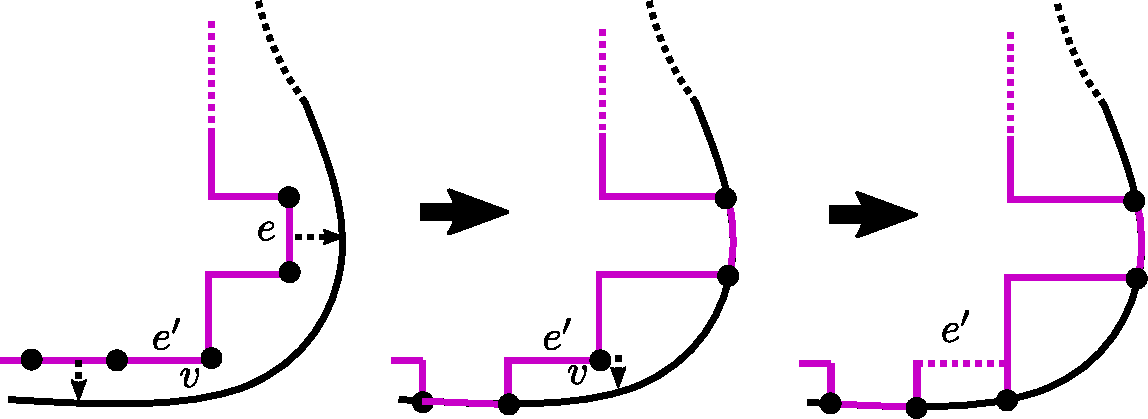
\includegraphics[width=\columnwidth]{general_geometry_extension_complete_Fig_1_crop}
  \caption{\label{fig:gengeomtryext}
    We project edge $e$ with vertices in $\mathbb{V}$ orthogonal to $e$ onto the boundary of $\mathbb{P}$.
    Project all such edges.
    Some vertices in $\mathbb{V}$ may not get projected.
    Suppose $v \in \mathbb{V}$  in print edge $e'$ is not projected (middle).
    Then convert $e'$ to idle movement in tool path, and project $v$ to the boundary of $\mathbb{P}$ orthogonal to $e'$ (right).
    Here, edge $e'$ could be idle to start with.
  }  	
\end{figure}

Implementation of the complete pipeline with IP mode (Section \ref{sec:ipmodel}) for a single layer is shown in Figure \ref{fig:singlebunnylayer}.
We can handle disconnected polygons, or ones with holes.
Figure \ref{fig:introimage} (in Page \pageref{fig:introimage}) and Figure \ref{fig:bunnybuddha} show sample layers from implementations on the Buddha and the Bunny. 
%It took approximately $40$ hours to generate the tool path.

\begin{figure*}[htp!] 
  \centering
  \begin{subfigure}[t]{2.16in}
    %\centering
    \hspace*{-0.4in}
    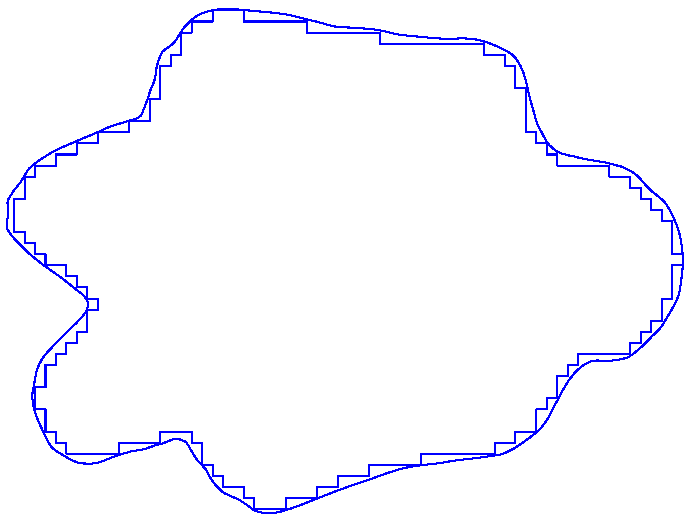
\includegraphics[scale=0.52]{bunny_layer_18_64_120_intorthAndGenpolygonimage_1_crop}
    \caption{\label{fig:singlebunnylayera}}
  \end{subfigure}
  \begin{subfigure}[t]{2.16in}
    %\centering
    \hspace*{-0.1in}
    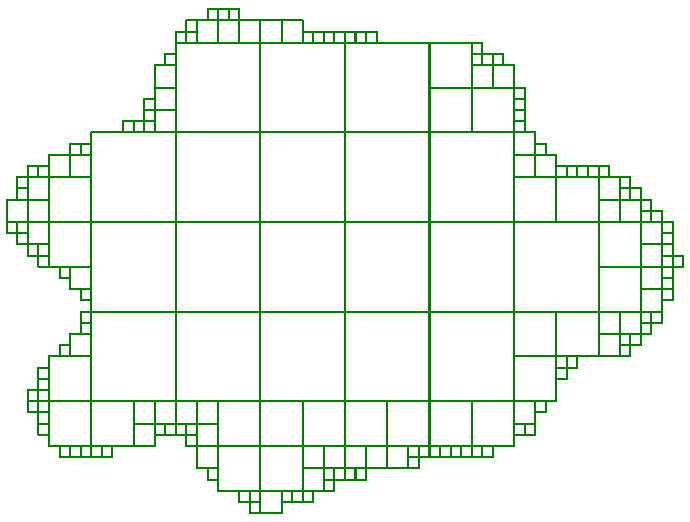
\includegraphics[scale=0.52]{bunny_layer_18_64_120_subsquareseqimage_1_crop}
    \caption{\label{fig:singlebunnylayerb}}
  \end{subfigure}
  \begin{subfigure}[t]{2.16in}
    %\centering
    \hspace*{-0.4in}
    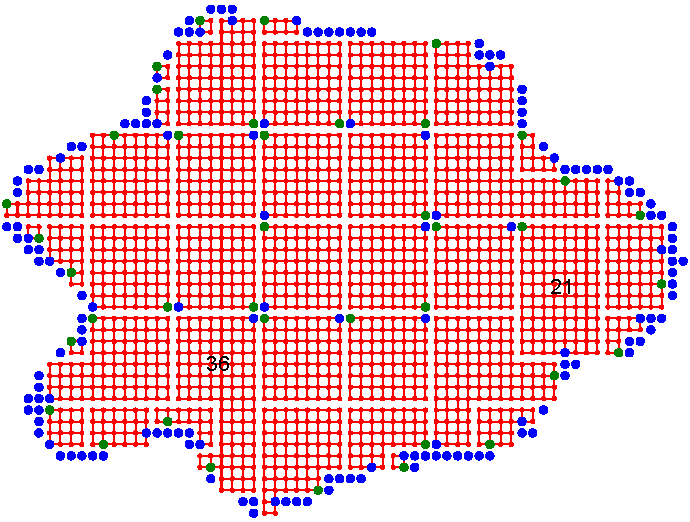
\includegraphics[scale=0.52]{bunny_layer_18_64_120_subsquareseqgraphseqimage_1_with_blocknumber_crop}
    \caption{\label{fig:singlebunnylayerc}}
  \end{subfigure}
  \begin{subfigure}[t]{2.16in}
    %\centering
    \hspace*{-0.1in}
    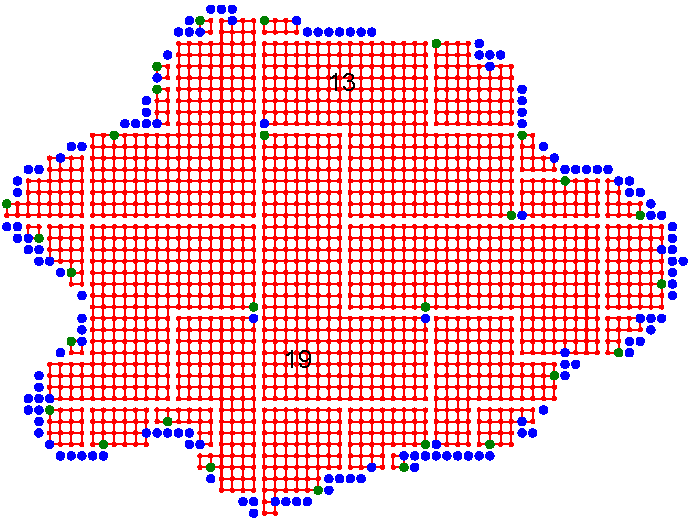
\includegraphics[scale=0.52]{bunny_layer_18_64_256_subsquareseqgraphseqimage_1_with_blocknumber_crop}
    \caption{\label{fig:singlebunnylayerd}}
  \end{subfigure}
  \begin{subfigure}[t]{2.16in}
    %\centering
    \hspace*{-0.4in}
    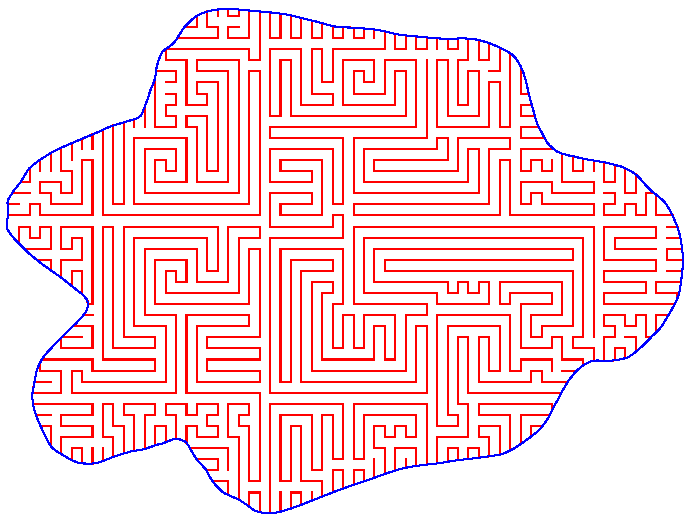
\includegraphics[scale=0.52]{bunny_layer_18_64_256_polygontoolpathimagewithgenpoly_1_crop}
    \caption{\label{fig:singlebunnylayere}}
  \end{subfigure}
  \begin{subfigure}[t]{2.16in}
    %\centering
    \hspace*{-0.1in}
    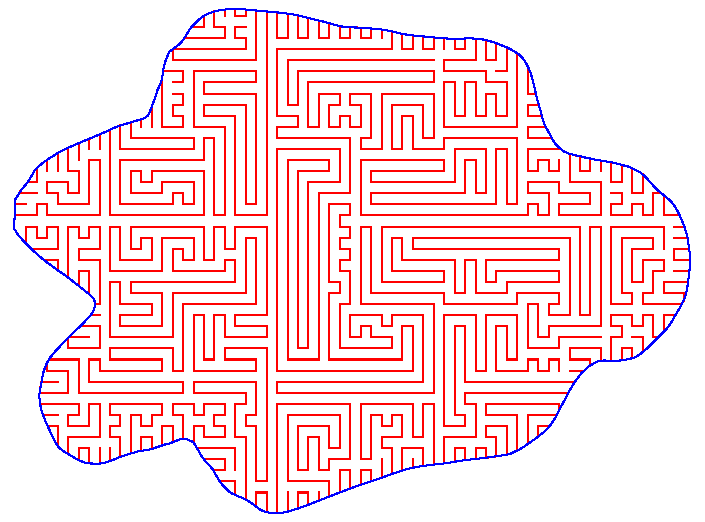
\includegraphics[scale=0.52]{bunny_layer_18_64_256_polygontoolpathimagewithgenpolywithrandomweight_1_crop}
    \caption{\label{fig:singlebunnylayerf}}
  \end{subfigure}	
  \caption{\label{fig:singlebunnylayer}
    Figure \ref{fig:singlebunnylayera} shows polygon $\mathbb{P}$ and its largest IOP $P$ in blue.
    Figure \ref{fig:singlebunnylayerb} shows decomposition of $P$ with $\delta = 64$.
    Figures \ref{fig:singlebunnylayerc} and \ref{fig:singlebunnylayerd} show dual graphs (red) after implementing Sections \ref{ssec:joincell}, \ref{ssec:enterexitvertexupdate} with $\Delta=120, 256$ (resp.).
    Enter and exit vertices are shown in green and blue dots (also isolated vertices).
    Print paths (red) with uniform and random edge weights are in Figures \ref{fig:singlebunnylayere} and \ref{fig:singlebunnylayerf} (both combined with turn costs).
    } 
\end{figure*}

\subsection{Maximizing or Minimizing Overlap} \label{ssec:maxminovlp}
We can maximize or minimize print edge overlap based on edge weights of adjacent layers.
To maximize (resp.~minimize) overlap, the weight of all edges in dual graph $\tilde{G}_i$ of Layer $i$ is set to $0.5$ (resp.~$1.5$) instead of $1$ (default), if they overlap with edges in print path of Layer $(i-1)$ (in the $xy$ plane).
Figure \ref{fig:maxminoverlapturnplot} shows variations of edge overlap ratios across the initial $148$ layers of Stanford Bunny. 
We make the following observations:
\begin{enumerate}
  \item\label{itm:maxminoverlapa}
    {\bfseries Figure \ref{fig:maxminoverlapturnplota}:}
    Original (uniform edge weights) and maximum overlap problems have similar overlap costs.
    For same $(\tilde{G}_i, s, t)$ between adjacent layers, both maximum overlap and original problems should return same solution.
    We can observe large changes in edge overlap at a few places in the original problem.
    It is due to significant variation in decompositions between adjacent layers.
    For instance, layers $33, 34, 35$ have significant differences in decomposition as shown in Figures \ref{fig:maxorivariationandminvariationa}, \ref{fig:maxorivariationandminvariationb}, \ref{fig:maxorivariationandminvariationc}.
    Further, the desired general trend of increase in overlap for maximum overlap and original problems, as well as decrease in overlap for minimum overlap, are observed due to increase in cross section area of the layers as we move up in $z$-axis.    

  \item\label{itm:maxminoverlapb}
    {\bf Figure \ref{fig:maxminoverlapturnplotb}:}
    In general there are sharp changes in number of turns across any $3$ adjacent layers in the minimum overlap problem, since it forces adjacent layers to have different tours.
    It further forces Layer $i+2$ to have similar toolpath as Layer $i$.
    This is illustrated for the same Block $5$ in layers $117, 118, 119$ in Figures \ref{fig:maxorivariationandminvariatione}, \ref{fig:maxorivariationandminvariationf}, \ref{fig:maxorivariationandminvariationg}. 
\end{enumerate}


\begin{figure*}[htp!] 
  \centering
  \begin{subfigure}[t]{3.25in}
    \centering
    %\hspace*{-0.5in}
    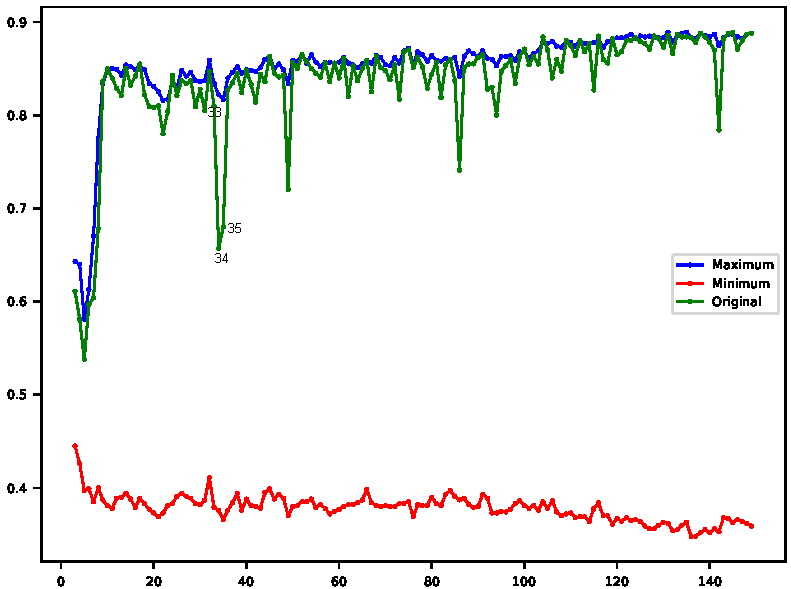
\includegraphics[scale=0.69]{MaxMinOriOverLapRatioPlot_crop_layer_label}
    \caption{\label{fig:maxminoverlapturnplota}}
  \end{subfigure}
  %\hfill
  \begin{subfigure}[t]{3.25in}
    \centering
    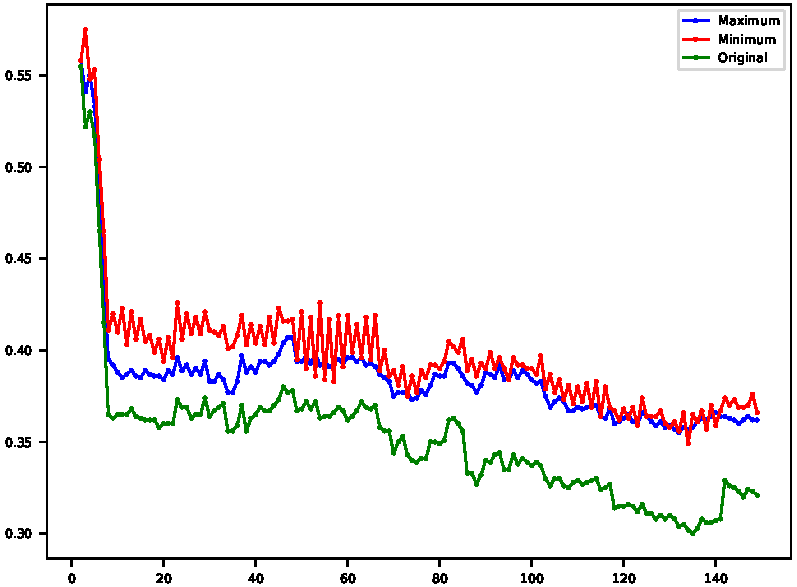
\includegraphics[scale=0.69]{MaxMinOriTurnRatioPlot_crop}
    \caption{\label{fig:maxminoverlapturnplotb}}
  \end{subfigure}
  \caption{\label{fig:maxminoverlapturnplot}
    Figure \ref{fig:maxminoverlapturnplota} shows Ratio (Total Overlapped printed edges / Total printed edges) vs Layer and Figure \ref{fig:maxminoverlapturnplotb} shows Ratio (Total 90 degree Turns / Total 90 and 180 degrees Turns) vs Layer for maximization, minimization, and using uniform edge weights (original) problems on the initial $148$ layers of the Bunny.
  }
\end{figure*}

\begin{figure*}[htp!] 
  \centering
  \begin{subfigure}[t]{2.1in}
    \centering
    \includegraphics[scale=0.45]{bunny_layer_33_64_256_subsquareseqgraphseqimage_1_crop}
    \caption{\label{fig:maxorivariationandminvariationa}}
  \end{subfigure}
  \begin{subfigure}[t]{2.1in}
    \centering
    \includegraphics[scale=0.45]{bunny_layer_34_64_256_subsquareseqgraphseqimage_1_crop}
    \caption{\label{fig:maxorivariationandminvariationb}}
  \end{subfigure}
  \begin{subfigure}[t]{2.1in}
    \centering
    \includegraphics[scale=0.45]{bunny_layer_35_64_256_subsquareseqgraphseqimage_1_crop}
    \caption{\label{fig:maxorivariationandminvariationc}}
  \end{subfigure}
  \begin{subfigure}[t]{2.1in}
    \centering
    \includegraphics[scale=0.45]{bunny_layer_117_64_256_subsquareseqgraphseqimage_1_blocknumber_crop}
    \caption{\label{fig:maxorivariationandminvariationd}}
  \end{subfigure}
  \hspace{1in}
  \begin{subfigure}[t]{1.5in}
    \centering
    \includegraphics[scale=0.63]{bunny_layer_117_64_256_subsquare_toolpath_minoverlap_block_5}
    \caption{\label{fig:maxorivariationandminvariatione}}
  \end{subfigure}
  \begin{subfigure}[t]{1.5in}
    \centering
    \includegraphics[scale=0.63]{bunny_layer_118_64_256_subsquare_toolpath_minoverlap_block_5}
    \caption{\label{fig:maxorivariationandminvariationf}}
  \end{subfigure}
  \begin{subfigure}[t]{1.5in}
    \centering
    \includegraphics[scale=0.63]{bunny_layer_119_64_256_subsquare_toolpath_minoverlap_block_5}
    \caption{\label{fig:maxorivariationandminvariationg}}
  \end{subfigure}
  \caption{\label{fig:maxorivariationandminvariation}
    Figures \ref{fig:maxorivariationandminvariationa}, \ref{fig:maxorivariationandminvariationb}, \ref{fig:maxorivariationandminvariationc} show decompositions for layers $33, 34, 35$ of the Bunny.
    Figure \ref{fig:maxorivariationandminvariationd} shows dual graph of layer $117$ with Block $5$ (present in layers $117, 118, 119$).
    Figures \ref{fig:maxorivariationandminvariatione}, \ref{fig:maxorivariationandminvariationf}, \ref{fig:maxorivariationandminvariationg} show tool path in those layers with minimum overlap on Block $5$.
  }
\end{figure*}


\begin{figure*}[hbp!] 
  \centering
  \includegraphics[height=2.02in]{bunnyLayer_125RenamedFrom124_image_256.png}
  \quad
  \includegraphics[height=2.02in]{bunnyLayer_312_image_256}\\
  \includegraphics[height=2.02in]{BuddhaTopImageLayer_90_256}
  \quad
  \includegraphics[height=2.02in]{BuddhaTopImageLayer_138_256.png}  
  \caption{\label{fig:bunnybuddha} Layers 125 and 312 of Bunny (top) and layers 90 and 138 of Buddha (bottom).}  	
\end{figure*}
\section{Mechanical Testing} \label{sec:mechtest}

We experimentally investigated the effects of space filling curve design and edge overlaps across adjacent layers on mechanical properties of the print.
We found that specimens with minimum and maximum edge overlaps have significantly different tensile behavior.

\subsection{Experimental Design and Fabrication}

Tensile specimens were shaped as the dog bone described by ASTM D638 \cite{astm2003}.
We modified its geometry slightly to exclude any sharp curvature boundaries.
The specimens had 40 layers at 0.2 mm layer height (Figure \ref{fig:dogbone}a).
We used a polyethylene terephthalate glycol-modified (PETG) filament of 1.75 mm in diameter in a desktop fused filament fabrication (FFF) device with a nozzle of 0.4 mm in diameter (from MatterHackers Inc., USA).
We used a universal tensile testing machine (INSTRON 600DX) in conjunction with an extensometer (Epsilon 3542-0200-50-ST) of 2'' gauge length, to measure tensile mechanical properties.
We performed the tests with a constant strain rate of 1.2 mm/minute.

Our space filling pattern has poorer bed adhesion than that of a conventional rectilinear raster pattern, hence the first layer was replaced with a 90$^\circ$ rectilinear pattern with 100\% density.
This first layer ensured good bed adhesion, and using just a single replacement layer minimized any effect on the sample’s tensile performance.
Printing the many orthogonal line segments with 90$^\circ$ turns with an extrusion width of 0.4 mm caused many holes to appear at the intersection of multiple extrusion corners.
Hence we extruded 10\% more material near a 90$^\circ$ turn in order to reduce the size and number of these holes.
We generated G-code for maximum and minimum overlap patterns (Figure \ref{fig:dogbone}b) and printed the specimens (Figure \ref{fig:dogbone}c).
The minimum overlap specimen took a significantly longer time to print than the maximum overlap specimen.
To investigate if the print time was affecting tensile properties, an additional maximum overlap specimen with reduced feed rate was fabricated to match the print time of the minimum overlap specimen.

We fabricated the specimens at a hot-end temperature of 235$^\circ$C, print-bed temperature of 75$^\circ$C, and extrusion speed of 30 mm/s.
Acceleration limit was set to 500 m/s$^2$.
The Linear Advance v1.5 feature from Marlin firmware was enabled to compensate for uneven extrusion due to speed variation.
For Linear Advance, a $k$-factor, which represents the length of filament compression needed per unit printing speed such that correct pressure is produced inside of the nozzle, was found experimentally to be 1.8.
%A 2 mm retraction was implemented throughout the toolpath and the overall number of retractions was minimized.

\begin{figure*}[htp!]
  \centering
  \includegraphics[width=\textwidth]{DogBone_DimsFailures.jpg}
  \caption{\label{fig:dogbone}
    Mechanical testing.
    a) Dog bone specimen dimensions in mm.
    b) Toolpath of a subdomain for maximum edge overlap.
    c) Final print of the subdomain.
    Failure surfaces shown for the maximum (d) and minimum (e) edge overlap cases are shown on the right, with specific features highlighted.
    }
\end{figure*}

\subsection{Results and Discussion}

Tensile test results and print times are shown in Table \ref{tab:dogboneResults}.
After the initial tensile test, the fracture surface suggested the presence of brittle failure in both the maximum and minimum overlap specimens (Figures \ref{fig:dogbone}d and \ref{fig:dogbone}e).

\begin{table}[htp!]
  \caption{  \label{tab:dogboneResults}
    Test results of dog bone specimens with maximum edge overlap (Max), maximum overlap printed with longer time (Max\_slow), and minimum edge overlap (Min).
    Strength gives the tensile strength in MPa, Elngtn give the elongation at break (as \%), Mdls gives the tensile modulus in GPa, and Time gives the print time in hours.
  }
  \centering
  \begin{tabular}{|l|c|c|c|c|} \hline
    Specimen & Strength & Elngtn & Mdls & Time  \\ \hline \hline
    Max & 20.0 & 1.09 & 1.81 & 19 \\ \hline
    Max\_slow & 23.8 & 1.28 & 1.86 & 28 \\ \hline
    Min & 32.9 & 1.62 & 1.85 & 28 \\ \hline
  \end{tabular}
\end{table}

The maximum edge overlap specimen failed  primarily due to localized delamination between the extrusion filaments \cite{DoJu2019} and exhibited line defects formed by connected air gaps (see Figure \ref{fig:dogbone}d).
The minimum edge overlap specimen experienced a catastrophic fracture.
The fracture surface of the slower print with maximum edge overlap exhibited a  fracture similar to that of the first maximum edge overlap specimen (as in Figure \ref{fig:dogbone}d), suggesting that the print time did not influence the experiments.
The maximum overlap specimen with normal feed rate has the smallest elongation at break and tensile strength.
The minimum overlap specimen has significantly large elongation at break and tensile strength.
%The slower feed rate may have improved tensile property for maximum overlap as shown in the stress-strain curve comparison in Fig **.

Overall, the stress-strain curves (Figure \ref{fig:dogboneStrStrCrvs}) reveal similarity in tensile moduli of the maximum and minimum overlap patterns. All
specimens experienced elongation at break and tensile strength less than the material specification.
The reduced elasticity could be due to the combined effect of intralayer adhesion arising from extrusion segment orientation \cite{ToRo2016}, and the type of dominant defects \cite{FaMoKa2019}  present as the result of different interlayer pattern generation strategy.
\begin{figure}[ht!]
  \centering
  \includegraphics[width=\columnwidth]{DogBone_StressStrainCurves.jpg}
  \caption{\label{fig:dogboneStrStrCrvs}
    Stress-Strain curves for maximum edge overlap (blue dashes), minimum edge overlap (red dots), and the maximum edge overlap with extended print time (green) specimens.
  }
\end{figure}

%Somewhat contrary to our initial expectation, the minimum overlap specimen exhibited higher strength under tensile load.
%This non-intuitive result may be due to how the layers are aggregated in each pattern.
%The maximum overlap pattern has layers of the same pattern stacked together, and the aforementioned holes are connected across layers, leading to line defects.
%Whereas the minimum overlap specimen has no two consecutive layers with the same pattern, limiting porous sites to individual vacancies instead of lines defects.

\section{Discussion}

We have developed a decomposition approach to solve large instances of optimized path planning problem in 3d printing where each sub-polygon is guaranteed to have a dual graph with a feasible tool path. 
Our framework guarantees that discontinuities in the tool path, if any, are located only at the boundary of the original (input) polygon.
Further, we can change the Hilbert ordering of the cells by changing enter and exit corner vertices of the initial cell in the quadtree.
We can also create various decompositions for the same IOP by changing parameters $\delta$ and $\Delta$.

The edge weights in our graphical framework could model multiple quality factors including turn costs, edge overlap across adjacent layers, tool path length, and others.
Our mechanical testing has shown that changing the extent of overlap across layers could impact the mechanical strength of the printed object.
Another potential application of our framework is the optimization of internal microstructure and thermal management by choosing appropriately defined edge weights derived from physical models and/or experiments, which in turn could result in increased strength of the printed objects.

For the Buddha and Bunny together, our framework solved more than 10,000 IP subproblems across more than 500 layers.
These IP instances could be solved independently, and hence in an embarrassingly parallel fashion.
Alternatively, our framework allows the use of approximation algorithms or heuristics to solve the subproblems instead of using IP \cite{ApBiChCo2007}.
We could also reuse optimal solutions for cells that reoccur across multiple layers.
Using uniform edge weights, and varying the relative importance parameter $\alpha$ (Equation \ref{eq:IPobj}), we could obtain fractal-like patterns for the toolpath.  

If we solve the full IP model (including subtour constraint \ref{eq:IPsubtr}), any discontinuities in the tool path are located at the boundary of the original polygon. 
This could be especially of concern when the polygon is relatively thin as compared to size of extruder.
We could consider reducing the extruder size to handle such situations, or consider alternative methods (e.g., spiral or zigzag patterns).
%\textcolor{blue}{With} relaxed IP model and associated heuristics, we cannot guarantee a single continuous path for each cell.
In extreme cases where the polygon in a given layer has many sharp curvature regions, we could have many small sized sub-polygons near the boundary.
This setting could create several discontinuities in the tool path at the boundary.
We will explore methods to handle such extreme cases in our future work.

Our mechanical testing experiments (Section \ref{sec:mechtest}), while preliminary, already demonstrate that the amount of edge overlap across adjacent layers could significantly affect the strength of the print.
We plan to employ the SFCDecomp framework to study in detail the effects of tool path design as well as edge overlap across layers on various mechanical properties.





